\documentclass{beamer}


\usepackage[utf8]{inputenc}
\usepackage{csquotes}
\usepackage{mdframed}
\usepackage{tensor}
\usepackage{xcolor}
\usepackage{amsthm}
\usepackage{amsmath}
\usepackage{mathtools}
\usepackage{amsfonts}
\usepackage{amssymb}
\usepackage{stmaryrd}
\usepackage{acro}
\usepackage{stmaryrd}
\usepackage{url}
\usepackage{tikz}
\usepackage{mathtools}
\usepackage{bussproofs}
\usepackage{syntax}
\usepackage[en-GB]{datetime2}
\usepackage[style=numeric,backend=bibtex]{biblatex}
\usepackage[final]{listings}
\usepackage{geometry}

\bibliography{bibliography}

\usetheme{m}

\setbeamertemplate{bibliography item}{\insertbiblabel}

\lstset{
	frame=lrtb,
	emph={while,fork,null,do,done,if,then,else,fi,skip,new,join},
	emphstyle=\textbf,
	mathescape,
	tabsize=3,
}

\newtheorem{defi}{Definition}
\renewenvironment{definition}
	{\begin{mdframed}[nobreak=true]\begin{defi}}
	{\end{defi}\end{mdframed}}


% -- tikz settings: --
\usetikzlibrary{arrows, cd, positioning, backgrounds, fit, decorations.pathmorphing, shapes.misc, calc}
\tikzset{%
	node/.style={draw, minimum size=8mm, inner sep=0mm, circle, fill=green!50},
	var/.style={draw, rectangle, minimum width=16mm, minimum height=6mm,%
		rounded corners=3pt, node distance=1cm, fill=purple!30},
	connector/.style={thick},
	sel/.style={->,thick},
	perm/.style={draw, rectangle},
	he/.style={draw, rectangle, minimum width=10mm, fill=blue!50},
	ext/.style={fill=brown!45},
	textnode/.style={draw, inner sep=4mm, rectangle, rounded corners=4pt}
}



\newcommand\irregularcircle[2]{% radius, irregularity
	let \n1 = {(#1)+rand*(#2)} in
	+(0:\n1)
	\foreach \a in {15,30,...,350}{
		let \n1 = {(#1)+rand*(#2)} in
		-- +(\a:\n1)
	} -- cycle
}


\newcommand{\Emb}{\mathit{Emb}}
\newcommand{\out}{\mathit{out}}
\newcommand{\fpHRG}{\mathit{fpHRG}_{\Sigma_{N}}^{\PI}}
\newcommand{\reach}{\mathit{reach}}
\newcommand{\FP}{\mathit{FP}}
\newcommand{\ap}{\mathit{ap}}
\newcommand{\fp}{\mathit{fp}}
\newcommand{\Proc}{\mathit{Proc}}
\newcommand{\emb}{\mathit{emb}}
\newcommand{\PI}{\mathit{Var}_{\text{process}}}
\newcommand{\rea}{\mathit{rea}}
\newcommand{\btr}{\blacktriangleright}
\newcommand{\type}{\mathit{type}}
\newcommand{\abs}{\mathit{abs}}
\newcommand{\br}{\mathit{br}}
\newcommand{\RB}{\mathit{RB}}
\newcommand{\NT}{\mathit{NT}}
\newcommand{\lhs}{\mathit{lhs}}
\newcommand{\rhs}{\mathit{rhs}}
\newcommand{\Tok}{\mathit{Tok}}
%\newcommand{\path}{\mathit{path}}
\newcommand{\Path}{\mathit{Path}}
\newcommand{\CPath}{\mathit{CPath}}
\newcommand{\AHC}{\mathit{AHC}_{\Sigma_{N}}^{\PI}}
\newcommand{\rk}{\mathit{rk}}
\newcommand{\con}{\mathit{con}}
\newcommand{\lab}{\mathit{lab}}
\newcommand{\ext}{\mathit{ext}}
\newcommand{\perm}{\mathit{perm}}
\newcommand{\HRG}{\mathit{HRG}_{\Sigma_{N}}^{\PI}}
\newcommand{\DSG}{\mathit{DSG}_{\Sigma_{N}}^{\PI}}
\newcommand{\HAG}{\mathit{HAG}_{\Sigma_{N}}^{\PI}}
\newcommand{\PES}{\mathit{PES}_{\PI}}
\newcommand{\HC}{\mathit{HC}_{\Sigma}^{\PI}}
\newcommand{\HCN}{\mathit{HC}_{\Sigma_{N}}^{\PI}}
\newcommand{\HG}{\mathit{HG}_{\Sigma}^{\PI}}
\newcommand{\HGN}{\mathit{HG}_{\Sigma_{N}}^{\PI}}
\newcommand{\aHG}{\mathit{HG}_{\Sigma_{N}}^{\PI}}
\newcommand{\HRule}{\rule{\linewidth}{0.5mm}}
\newcommand{\Sel}{\mathit{Sel}}
\newcommand{\Var}{\mathit{Var}}
\newcommand{\enum}{\mathit{enum}}
\newcommand{\Cont}{\mathit{Cont}}
\newcommand{\afiso}{\tensor[_\ap]{\cong}{_\fp}}
\newcommand{\border}{\mathit{border}}
\newcommand{\img}{\mathit{img}}
\newcommand{\off}{\mathit{offspring}}




\newcommand\blfootnote[1]{%
	\begingroup
	\renewcommand\thefootnote{}\footnote{#1}%
	\addtocounter{footnote}{-1}%
	\endgroup
}

%acronyms:
\DeclareAcronym{HAG}{
	short = HAG,
	long  = Heap Abstraction Grammar
}
\DeclareAcronym{AHC}{
	short = AHC,
	long  = admissible heap configuration
}
\DeclareAcronym{DSG}{
	short = DSG,
	long  = data structure grammar
}
\DeclareAcronym{HG}{
	short = HG,
	long  = hypergraph
}

\DeclareAcronym{HC}{
	short = HC,
	long  = heap configuration
}

\DeclareAcronym{HRG}{
	short = HRG,
	long  = hyperedge replacement grammar
}

\DeclareAcronym{fpHRG}{
	short = fpHRG,
	long  = fully permissive HRG
}

\DeclareAcronym{HR}{
	short = HR,
	long  = hyperedge replacement
}

\DeclareAcronym{PE}{
	short = PE,
	long  = permission expression
}

\DeclareAcronym{PES}{
	short = PES,
	long  = permission expression set
}

\DeclareAcronym{PM}{
	short = PM,
	long  = permission model
}

\DeclareAcronym{HM}{
	short = HM,
	long  = hypergraph morphismen
}





\title{Thread-Modular Analysis of Heap-Manipulating Programs}
\subtitle{Bachelor Colloquium}
\date{\DTMdisplaydate{2015}{8}{27}{-1}}
\author{Christoph Welzel}
\institute{Lehrstuhl für Informatik 2}

\metroset{everytitleformat=regular, numbering=fraction}

\begin{document}
\maketitle

\section{Introduction}
%
\begin{frame}
	\frametitle{Introduction}
	\begin{columns}
		\column{0.5\textwidth}
		\begin{itemize}
			\item software relies on:
				\begin{itemize}
					\item dynamic allocation of objects
					\item pointer
				\end{itemize}
			\item to build data-structures:
				\begin{itemize}
					\item binary trees
					\item (doubly, singly) linked lists
					\item \dots
				\end{itemize}
			\item[$\Rightarrow$] representation by graphs
		\end{itemize}
		\onslide<2-3>{\alt<2>{
			\column{0.5\textwidth}
			\resizebox{\textwidth}{!}{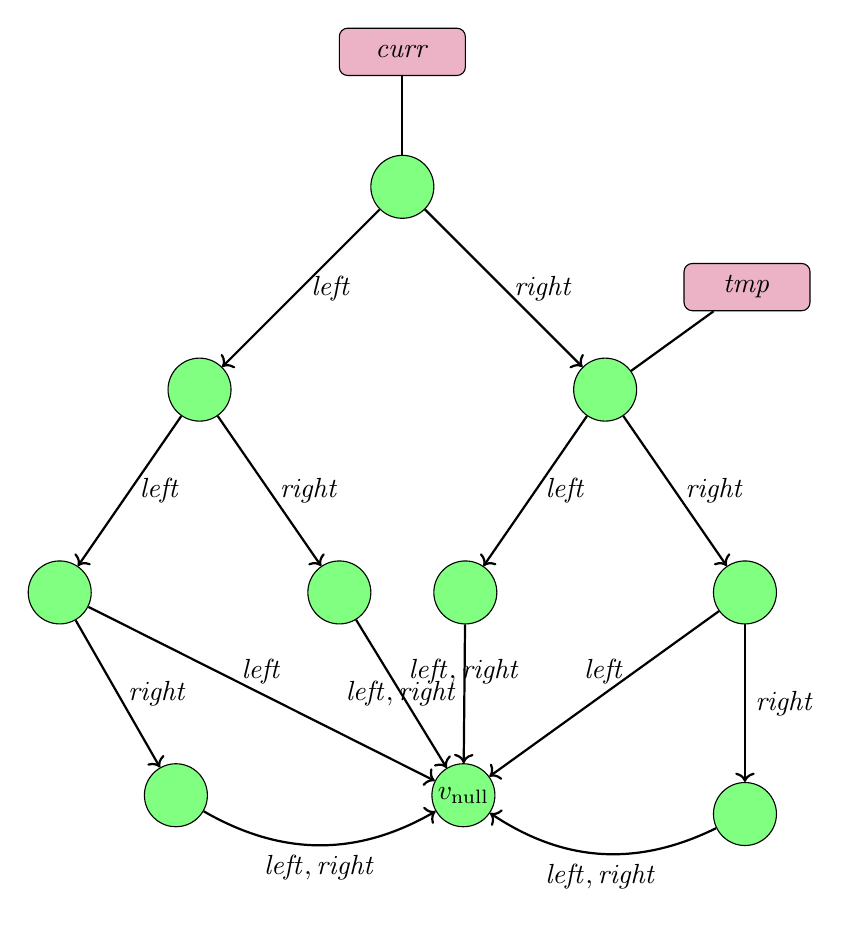
\begin{tikzpicture}[node distance=2 and 2]
		\node[node] (r)  {};
		\node[var] (curr) [above=of r] {$\mathit{curr}$};
		\node[node] (r-l) [below left=of r] {};
		\node[node] (r-r) [below right=of r] {};
		\node[node, node distance=2 and 1.2] (r-l-l) [below left=of r-l] {};
		\node[node, node distance=2 and 1.2] (r-l-r) [below right=of r-l] {};
		\node[node, node distance=2 and 1.2] (r-r-l) [below left=of r-r] {};
		\node[node, node distance=2 and 1.2] (r-r-r) [below right=of r-r] {};
		\node[node]                          (r-r-r-r) [below=of r-r-r] {};
		\node[node, node distance=2 and 0.9] (r-l-l-r) [below right=of r-l-l] {};
		\node[var] (tmp)  [above right=of r-r] {$\mathit{tmp}$};
		\node[node, below right=2 and 1 of r-l-r] (null) {$v_{\text{null}}$};
		\draw [connector] (tmp) to (r-r);
		\draw [connector] (curr) to (r);
		\draw [sel] (r) to node[right]{$\mathit{left}$} (r-l) ;
		\draw [sel] (r) to node[right]{$\mathit{right}$} (r-r);
		\draw [sel] (r-l) to node[right]{$\mathit{left}$} (r-l-l);
		\draw [sel] (r-l) to node[right]{$\mathit{right}$} (r-l-r);
		\draw [sel] (r-r) to node[right]{$\mathit{left}$} (r-r-l);
		\draw [sel] (r-r) to node[right]{$\mathit{right}$} (r-r-r);
		\draw [sel] (r-r-r) to node[right]{$\mathit{right}$} (r-r-r-r);
		\draw [sel] (r-l-l) to node[right]{$\mathit{right}$} (r-l-l-r);
		\draw [sel] (r-l-l) to node[above]{$\mathit{left}$} (null);
		\draw [sel] (r-r-r) to node[above]{$\mathit{left}$} (null);
		\draw [sel] (r-l-r) to node{$\mathit{left},\mathit{right}$} (null);
		\draw [sel] (r-r-l) to node[above]{$\mathit{left},\mathit{right}$} (null);
		\draw [sel, bend left] (r-r-r-r) to node[below]{$\mathit{left},\mathit{right}$} (null);
		\draw [sel, bend right] (r-l-l-r) to node[below]{$\mathit{left},\mathit{right}$} (null);

	\end{tikzpicture}
}
		}{
			\column{0.5\textwidth}
			\begin{itemize}
				\item parallel execution
					\begin{itemize}
						\item \emph{Go}:
							\enquote{explicit support for concurrent programming}
						\item possible data races
					\end{itemize}
			\end{itemize}
	}}
	\end{columns}
	\blfootnote{\cite{golang}}
\end{frame}

\begin{frame}
	\frametitle{Contribution}
	\begin{itemize}
		\item analysis to work on graph representation with explicit support for
			parallel execution
			\begin{itemize}
				\item \alert<2>{ensures data race freedom}
				\item \alert<3>{ensures absence of null pointer dereferences}
				\item \alert<4>{enables checking correctness}
			\end{itemize}
	\end{itemize}
\end{frame}

\begin{frame}
	\frametitle{Table of Contents}
	\tableofcontents
\end{frame}

\metroset{numbering=none}
\section{Programming Language}

\metroset{numbering=fraction}

\begin{frame}
	\frametitle{Features}
	\begin{columns}
		\column{0.5\textwidth}
		\begin{itemize}
			\item \emph{Java}-like
				\begin{itemize}
					\item (implicitly) garbage collected
					\item object oriented
					\item objects are universally typed
				\end{itemize}
		\end{itemize}
		\begin{itemize}
			\item parallel execution
				\begin{itemize}
					\item \emph{fork}: implicit \emph{process} creation
					\item \emph{join}: synchronisation on termination (optional)
				\end{itemize}
		\end{itemize}
		\column{0.5\textwidth}
		\onslide<2>{\scalebox{0.7}{\begin{tikzpicture}
	\node[rectangle, draw] (m) {\underline{Main}};
	\node[rectangle, draw, minimum width=0.5cm, minimum height=5cm, below=0.5 of m] (am) {};
	\node[rectangle, draw, below right=1 and 1 of m, minimum width=1.2cm] (p1) {\underline{$P_1$}};
	\node[rectangle, draw, below left=2 and 1 of m, minimum width=1.2cm] (p2) {\underline{$P_2$}};
	\node[rectangle, draw, below right=of p1, minimum width=1.2cm, minimum height=0.7cm] (other) {\dots};
	\node[rectangle, draw, minimum width=0.5cm, minimum height=2cm, below=0.5 of p1] (p1m) {};
	\node[circle, cross out, below=0.5 of p1m, minimum width=0.5cm, draw, minimum height=0.5cm] (p1e) {};
	\node[rectangle, draw, minimum width=0.5cm, minimum height=1.5cm, below=0.5 of p2] (p2m) {};
	\node[circle, cross out, below=0.5 of p2m, minimum width=0.5cm, draw, minimum height=0.5cm] (p2e) {};
	\node[below=0.3cm of am] (me) {};

	\draw[dashed] (m) to (am);
	\draw[->] ([yshift=1.67cm]am.east) to node[above]{\small fork} (p1);
	\draw[->] ([yshift=0.67cm]am.west) to node[above]{\small fork} (p2);
	\draw[->] ([yshift=0.16cm]p1m.east) to node[above]{\small fork} (other);
	\draw[dashed] (p1) to (p1m);
	\draw[dashed] (p1m.south) to (p1e.center);
	\draw[dashed] (p2) to (p2m);
	\draw[dashed] (p2m.south) to (p2e.center);
	\draw[->] (p1e.center) to node[above]{\small join} ([yshift=0.57cm]am.south east);
	\draw[dashed] (am) to (me);
\end{tikzpicture}
}}
	\end{columns}
\end{frame}

\begin{frame}[fragile]
	\frametitle{Syntax}
	Context:
	\begin{columns}
		\column{0.5\textwidth}
			\begin{itemize}
				\item $\Var$ - Variables
				\item $\Sel$ - Selectors
			\end{itemize}
		\column{0.5\textwidth}
			\begin{itemize}
				\item $\Proc$ - Programs
				\item $\PI$ - Process Identifier
			\end{itemize}
	\end{columns}
	\setlength{\grammarindent}{2cm}
	\begin{grammar}
	<P> ::= \textbf{null} | $x$ | $x.s$

	<S> ::= $x$=<P> | $x.s$ = <P> | \textbf{new}($x$) |
	$t$=\textbf{fork}$(m(x_1,\dots,x_n))$ | join($t$) | $t_1 = t_2$
	\end{grammar}
\end{frame}

\begin{frame}[fragile]
	\frametitle{Example}
	\begin{columns}
		\column{0.55\textwidth}
		\begin{lstlisting}
while($\mathit{curr.left}$ != null) do
	$\mathit{tmp}$ = $\mathit{curr.right}$;
	$t$ = fork($\mathit{traverse}$($\mathit{tmp}$));
	$\mathit{curr}$ = $\mathit{curr.left}$;
done;
$\mathit{tmp} = \mathit{curr.right}$;
$t$ = fork($\mathit{traverse}$($\mathit{tmp}$));
$\mathit{tmp} = $ null;
join($t$);
$\mathit{curr.left} = \mathit{curr.right}$;
$\mathit{curr.right} = $ null;
			\end{lstlisting}
		\column{0.45\textwidth}
		\only<1>{\begin{itemize}
				\item $\Proc = \{ \mathit{traverse} \}$
				\item $\Sel  = \{ \mathit{left}, \mathit{right} \}$
				\item $\Var  = \{ \mathit{curr}, \mathit{tmp}   \}$
				\item $\PI   = \{ t \}$
			\end{itemize}
		}
		\only<2>{
			\resizebox{\textwidth}{!}{\input{tikz/BinTreeEx1}}
		}
		\only<3>{
			\resizebox{\textwidth}{!}{\input{tikz/BinTreeEx2}}
		}
		\only<4>{
			\resizebox{\textwidth}{!}{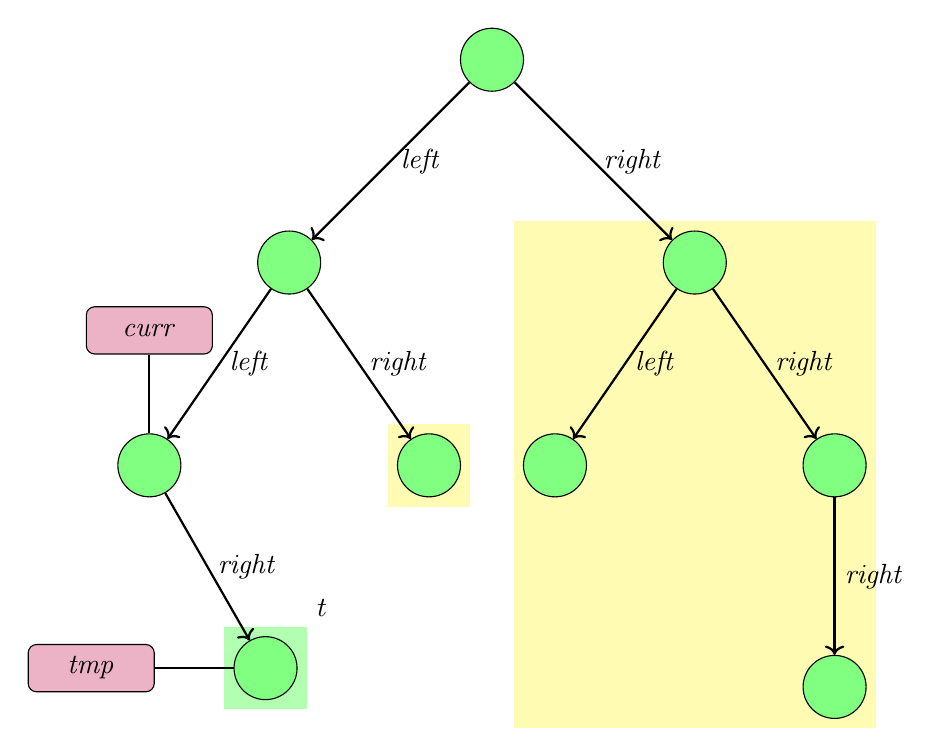
\begin{tikzpicture}[node distance=2 and 2]
			\node[node] (r)  {};
			\node[node] (r-l) [below left=of r] {};
			\node[node] (r-r) [below right=of r] {};
			\node[node, node distance=2 and 1.2] (r-l-l) [below left=of r-l] {};
			\node[var] (curr) [above =of r-l-l] {$\mathit{curr}$};
			\node[node, node distance=2 and 1.2] (r-l-r) [below right=of r-l] {};
			\node[node, node distance=2 and 1.2] (r-r-l) [below left=of r-r] {};
			\node[node, node distance=2 and 1.2] (r-r-r) [below right=of r-r] {};
			\node[node]                          (r-r-r-r) [below=of r-r-r] {};
			\node[node, node distance=2 and 0.9] (r-l-l-r) [below right=of r-l-l] {};
			\node[var, left=of r-l-l-r] (tmp) {$\mathit{tmp}$};
			\draw [connector] (tmp) to (r-l-l-r);
			\draw [connector] (curr) to (r-l-l);
			\draw [sel] (r) to node[right]{$\mathit{left}$} (r-l);
			\draw [sel] (r) to node[right]{$\mathit{right}$} (r-r);
			\draw [sel] (r-l) to node[right]{$\mathit{left}$} (r-l-l);
			\draw [sel] (r-l) to node[right]{$\mathit{right}$} (r-l-r);
			\draw [sel] (r-r) to node[right]{$\mathit{left}$} (r-r-l);
			\draw [sel] (r-r) to node[right]{$\mathit{right}$} (r-r-r);
			\draw [sel] (r-r-r) to node[right]{$\mathit{right}$} (r-r-r-r);
			\draw [sel] (r-l-l) to node[right]{$\mathit{right}$} (r-l-l-r);

			\begin{scope}[on background layer]
				\node [fill=yellow!30,fit=(r-r) (r-r-r) (r-r-l) (r-r-r-r)] {};
			\end{scope}
			\begin{scope}[on background layer]
				\node [fill=yellow!30,fit=(r-l-r)] {};
			\end{scope}
			\begin{scope}[on background layer]
				\node [fill=green!30,fit=(r-l-l-r), label=45:$t$] {};
			\end{scope}
		\end{tikzpicture}
}
		}
		\only<5>{
			\resizebox{\textwidth}{!}{\input{tikz/BinTreeEx4}}
		}
		\end{columns}
\end{frame}

\section{Permission Model}
\begin{frame}
	\frametitle{Idea}
	\begin{itemize}
		\item add access rights to values
			\begin{itemize}
				\item introduce access tickets
				\item account for derived tickets for forked processes
			\end{itemize}
		\item ensure:
			\begin{itemize}
				\item shared access restricts to reading
				\item write access is exclusive
			\end{itemize}
	\end{itemize}
	\blfootnote{\cite{SeparationLogic}, \cite{MultithreadedJavaPrograms}}
\end{frame}

\begin{frame}
	\frametitle{Considerations}
	\begin{columns}
		\column{0.5\textwidth}
		\begin{itemize}
			\item distinguish \emph{write} \& \emph{read} access:
				\begin{itemize}
					\item $\mathit{WR}$
					\item $\mathit{RD}$
				\end{itemize}
			\item account for derived read access
			\item transfer write access completely
			\item<3-> potential loss of information about access:
				\begin{itemize}
					\item<3-> $\mathit{WR}^{\ast}$
					\item<3-> $\mathit{RD}^{\ast}$
				\end{itemize}
		\end{itemize}
		\column{0.5\textwidth}
		\only<2->{\resizebox{\textwidth}{!}{\input{tikz/BinTreeEx2}}}
	\end{columns}
	\blfootnote{\cite{FractionalPermissions}}
\end{frame}

\begin{frame}
	\frametitle{Permission Expression}
	\begin{itemize}
		\item through assignment multiple process identifier refer to same
			process
		\item[$\Rightarrow$] token: $T\in\mathbb{P}(\PI)$
	\end{itemize}
	\pause
	\begin{definition}[Permission Expression]
		\begin{equation*}
			\underbrace{\mathit{BasePerm}}_{\in\left\{\mathit{WR}, \mathit{RD},
			\mathit{WR}^{\ast}, \mathit{RD}^{\ast}\right\}} -
			\underbrace{\mathit{PermSet}}_{\subseteq\mathbb{P}(\PI)}
		\end{equation*}
	\end{definition}
\end{frame}

\begin{frame}
	\frametitle{Placeholders}
		\begin{overlayarea}{\textwidth}{\textheight}
			\begin{columns}
				\column{0.5\textwidth}
				\begin{itemize}
					\item add token for read access
				\end{itemize}
				\uncover<2->{\resizebox{\textwidth}{!}{\input{tikz/BinTreeProgLangPerm}}}
				\column{0.5\textwidth}
				\begin{itemize}
					\item replace by placeholder for write access
				\end{itemize}
				\uncover<3>{\resizebox{\textwidth}{!}{\begin{tikzpicture}[node distance=2 and 2]
	\node[node] (r)  {};
	\node[var] (curr) [above=of r] {$\mathit{curr}$};
	\node[node] (r-l) [below left=of r] {};
	\node[node] (r-r) [below right=of r] {};
	\node[node, node distance=2 and 1.2] (r-l-l) [below left=of r-l] {};
	\node[node, node distance=2 and 1.2] (r-l-r) [below right=of r-l] {};
	\node[node, node distance=2 and 1.2] (r-r-l) [below left=of r-r] {};
	\node[node, node distance=2 and 0.9] (r-l-l-r) [below right=of r-l-l] {};
	\node[he, node distance=2 and 0.9] (Nt) [below right=of r-r] {$N_{\{t\}}$};
	\node[node, below right=2 and 1 of r-l-r] (null) {$v_{\text{null}}$};
	\draw [connector] (curr) to (r);
	\draw [connector] (r-r) to (Nt);
	\draw [connector, bend left=50] (Nt) to (null);
	\draw [sel] (r) to node[left]{$l_{\mathit{WR}}$} (r-l) ;
	\draw [sel] (r) to node[right]{$r_{\mathit{WR}}$} (r-r);
	\draw [sel] (r-l) to node[left]{$l_{\mathit{WR}}$} (r-l-l);
	\draw [sel] (r-l) to node[right]{$r_{\mathit{WR}}$} (r-l-r);
	\draw [sel] (r-r) to node[right] {$l_{\mathit{WR} - \{\{t\}\}}$} (r-r-l);
	\draw [sel] (r-l-l) to node[right]{$r_{\mathit{WR}}$} (r-l-l-r);
	\draw [sel] (r-l-l) to node[above]{$l_{\mathit{WR}}$} (null);
	\draw [sel] (r-l-r) to node{$(l,r)_{\mathit{WR}}$} (null);
	\draw [sel] (r-r-l) to node[above right]{$(l,r)_{\mathit{WR} - \{\{t\}\}}$}
		(null);
	\draw [sel, bend right] (r-l-l-r) to node[below]{$(l,r)_{\mathit{WR}}$}
		(null);

	\begin{scope}[on background layer]
		\node[fill=green!30,fit=(r-r) (r-r-r) (r-r-l) (r-r-r-r),label=125:$t$]{};
	\end{scope}
\end{tikzpicture}

}}
			\end{columns}
		\end{overlayarea}
\end{frame}

\section{Hypergraphs}
\begin{frame}
	\frametitle{Intuition}
	\begin{itemize}
		\item hypergraphs allow edges to connect arbitrary many nodes
		\item modelling heap structure as hypergraphs:
	\end{itemize}
	\begin{columns}
		\column{0.5\textwidth}
			\begin{itemize}
				\item objects as nodes
				\item variables as unary hyperedges
				\item selectors as binary hyperedges
				\item placeholders as hyperedges with arbitrary many nodes
			\end{itemize}
		\column{0.5\textwidth}
			\resizebox{\textwidth}{!}{\input{tikz/hgexp1}}
	\end{columns}
	\blfootnote{\cite{InformalGraphGrammars}}
\end{frame}

\begin{frame}
	\frametitle{Hyperedge Replacement}
	\begin{itemize}
		\item re-integrate \enquote{$\mathit{WR}$-part} upon join
		\item replace hyperedge by hypergraph
		\item instructions can have the form of production rules:
	\end{itemize}
	\begin{center}
		\resizebox{0.5\textwidth}{!}{
			\begin{tikzpicture}
				\node[he] (lhs) {$N_{\{t\}}$};
				\node[right=2 and 2 of lhs] (rhs) {\scalebox{0.7}{\input{tikz/presprod}}};
				\draw[->, thick, shorten <= 0.5cm, shorten >= 0.5cm] (lhs) to (rhs);
			\end{tikzpicture}
		}
	\end{center}
	\blfootnote{\cite[p. 104]{HandbookGraphGrammars}}
\end{frame}

\begin{frame}
	\frametitle{Example}
	\resizebox{0.3\textwidth}{!}{\begin{tikzpicture}
				\node[he] (lhs) {$N_{\{t\}}$};
				\node[right=2 and 2 of lhs] (rhs) {\scalebox{0.7}{\input{tikz/presprod}}};
				\draw[->, thick, shorten <= 0.5cm, shorten >= 0.5cm] (lhs) to (rhs);
			\end{tikzpicture}}
			\flushright\visible<2->{\resizebox{!}{5cm}{
	\begin{tikzpicture}
			\node (pre) {\scalebox{0.6}{\begin{tikzpicture}[node distance=2 and 2]
	\node[node] (r)  {};
	\node[var] (curr) [above=of r] {$\mathit{curr}$};
	\node[node] (r-l) [below left=of r] {};
	\node[node, fill=gray!50] (r-r) [below right=of r] {};
	\node[node, node distance=2 and 1.2] (r-l-l) [below left=of r-l] {};
	\node[node, node distance=2 and 1.2] (r-l-r) [below right=of r-l] {};
	\node[node, node distance=2 and 1.2] (r-r-l) [below left=of r-r] {};
	\node[node, node distance=2 and 0.9] (r-l-l-r) [below right=of r-l-l] {};
	\node[node, below right=2 and 1 of r-l-r, fill=gray!50] (null) {$v_{\text{null}}$};
	\node[var] (tmp)  [above right=of r-r] {$\mathit{tmp}$};
	\node[he] (p) [below right=2 and 1.2 of r-r] {$N_{\{t\}}$};
	
	\node[node, ext] (r-r2) [below right =0.6 and 0.6 of null] {$v_{1}$};
	\node[node, node distance=2 and 1.2] (r-r-r) [below right=of r-r2] {$v_{3}$};
	\node[node]                          (r-r-r-r) [below=1.2 and 1.2 of r-r-r] {$v_{4}$};
	\node[node, ext, node distance=3 and 1.2] (null2)    [below=of r-r2] {$v_{\textbf{null}}$};

	\draw [sel] (r-r2) to node[right, label={180:$e_{2}$}]{$r_{\mathit{WR}}$} (r-r-r);
	\draw [sel] (r-r-r) to node[right, label={180:$e_{3}$}]{$l_{\mathit{WR}}$} (r-r-r-r);
	\draw [sel] (r-r-r) to node[above left, label={[label distance=-2mm]0:$e_{4}$}]{$r_{\mathit{WR}}$} (null2);
	\draw [sel] (r-r-r-r) to node[above,label={[label distance=-1mm]-90:$e_{7}$}]{$r_{\mathit{WR}}$} (null2);
	\draw [sel, bend left] (r-r-r-r) to node[below, label={[label distance=-2mm]180:$e_{8}$}]{$l_{\mathit{WR}}$} (null2);

	\draw [connector] (tmp) to (r-r);
	\draw [connector] (curr) to (r);
	\draw [connector] (p) to (r-r);
	\draw [connector, bend left] (p) to (null);
	\draw [sel] (r) to node[left]{$l_{\mathit{WR}}$} (r-l) ;
	\draw [sel] (r) to node[right]{$r_{\mathit{WR}}$} (r-r);
	\draw [sel] (r-l) to node[left]{$l_{\mathit{WR}}$} (r-l-l);
	\draw [sel] (r-l) to node[right]{$r_{\mathit{WR}}$} (r-l-r);
	\draw [sel] (r-r) to node[right, label={[label distance=0mm]-90:$l_{\mathit{WR}}$}]{} (r-r-l);
	\draw [sel] (r-l-l) to node[right]{$r_{\mathit{WR}}$} (r-l-l-r);
	\draw [sel] (r-l-l) to node[above]{$l_{\mathit{WR}}$} (null);
	\draw [sel] (r-l-r) to node{$(l,r)_{\mathit{WR}}$} (null);
	\draw [sel] (r-r-l) to node[above right]{$(l,r)_{\mathit{WR}}$} (null);
	\draw [sel, bend right] (r-l-l-r) to node[below]{$(l,r)_{\mathit{WR}}$} (null);

	\draw [->, dashed, bend right] (r-r2) to (r-r);
	\draw [->, dashed, bend left] (null2) to (null);
\end{tikzpicture}
}};
			\visible<3>{\node[right=of pre] (t) {$\Rightarrow$};
			\node[right=of t] (post) {\scalebox{0.7}{\input{tikz/forkexample10}}};}
		\end{tikzpicture}
	}}
\end{frame}

\section{Semantics}
\begin{frame}
	\frametitle{Introduction}
	\begin{itemize}
		\item model behaviour of statements as graph transformations
		\item every statement for which no behaviour is modelled explicitly yields
			a \emph{fault} symbol
		\item[1.] pointer assignments:
			\begin{itemize}
				\item \alert{for selectors ensure that the permission is
					$\mathit{WR} - \emptyset$}
				\item connect assigned selector or variable accordingly
			\end{itemize}
		\item[2.] allocation:
			\begin{itemize}
				\item add new node to hypergraph
				\item add all selectors for node, point them to $v_{\text{null}}$
				\item \alert{every new selector holds $\mathit{WR}-\emptyset$}
			\end{itemize}
		\item[3.] \alert{process identifier assignment ($t = t'$):}
			\begin{itemize}
				\item \alert{remove $t$ from tokens (for
					a singleton token $\{t\}$ \enquote{star} $\mathit{BasePerm}$,
				remove placeholder)}
				\item \alert{add $t$ to tokens containing $t'$}
			\end{itemize}
	\end{itemize}
\end{frame}

\begin{frame}
	\frametitle{Fork}
	\begin{itemize}
		\item actual vs. formal parameters
		\item forked programs behave according to contracts:
			\begin{itemize}
				\item precondition: context of forking process (encodes actual
					parameters)
				\item alterable set: selectors that can be altered
				\item postcondition: result of computation of forked process
			\end{itemize}
	\end{itemize}
	\begin{equation*}
		\Cont\colon\Proc\rightarrow\mathbb{P}(
		\underbrace{\HG}_{\text{precondition}}\times
		\underbrace{\mathbb{P}(E)}_{\text{alterable set}}\times
		\underbrace{\mathit{HG}^{\PI'}_{\Sigma'}}_{\text{postcondition}})
	\end{equation*}
	\begin{equation*}
		\left(\parbox{2cm}{\resizebox{2cm}{!}{\input{tikz/precondition}}},
			\{e_2,e_3,e_4, e_7, e_8\},
		\parbox{2cm}{\resizebox{2cm}{!}{\input{tikz/postcondition}}}\right)
	\end{equation*}
\end{frame}

\begin{frame}
	\frametitle{Fork}
	$t = \textbf{fork}(m(x_{1},\dots,x_{n}));$
	\begin{itemize}
		\item find fitting contract:
			\begin{enumerate}
				\item compute reachable subgraph from actual parameters
					($x_1,\dots,x_n$)
				\item match with precondition
				\item compute border nodes
				\item ensure forked and forking process agree on border nodes
			\end{enumerate}
		\item<2-> apply contract:
			\begin{enumerate}
				\item free the assigned process identifier ($t$)
				\item remove selectors from alterable set in heap representation of
					forking process
				\item add placeholder connected to border nodes ($N_{\{t\}}$)
				\item add token of newly forked process ($\{t\}$) to
					$\mathit{PermSets}$ of reachable subgraph
			\end{enumerate}
	\end{itemize}
\end{frame}

\begin{frame}
	\frametitle{Example}
	\begin{columns}
		\column{0.5\textwidth}
			\begin{equation*}
				\alt<1>{\left(\parbox{2cm}{\resizebox{2cm}{!}{
						\input{tikz/precondition}}}, \{e_2,e_3,e_4, e_7, e_8\},
				\parbox{2cm}{\resizebox{2cm}{!}{\input{tikz/postcondition}}}\right)
			}{
				\alt<2-7>{\parbox{2cm}{\resizebox{2cm}{!}{\input{tikz/precFork1}}}}
				{\parbox{2cm}{\resizebox{2cm}{!}{\input{tikz/precFork2}}}}
			}
			\end{equation*}
			\visible<3->{
				\begin{enumerate}
					\item \alert<5>{compute reachable subgraph from actual
						parameters}
					\item \alert<6>{match with precondition}
					\item \alert<7>{compute border nodes}
					\item \alert<8>{ensure forked and forking process agree on
							border nodes}
				\end{enumerate}
			}
		\column{0.5\textwidth}
		\begin{overlayarea}{\textwidth}{\textheight}
		\vspace{1.5cm}
			\only<4>{
				\resizebox{\textwidth}{!}{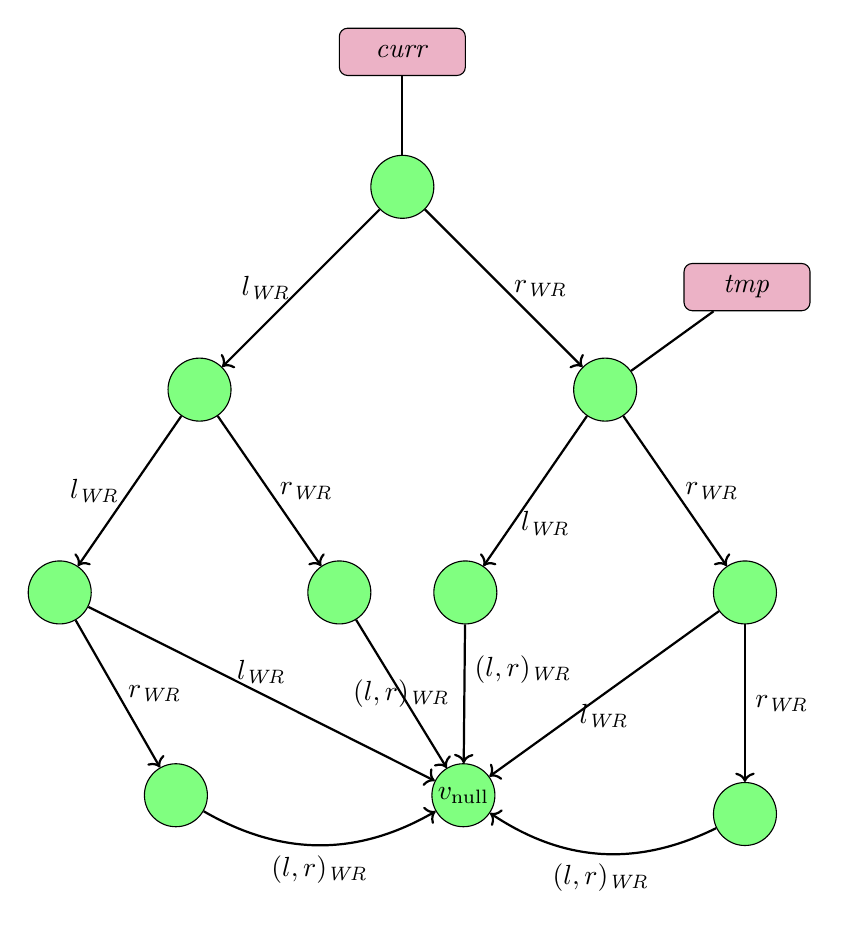
\begin{tikzpicture}[node distance=2 and 2]
	\node[node] (r)  {};
	\node[var] (curr) [above=of r] {$\mathit{curr}$};
	\node[node] (r-l) [below left=of r] {};
	\node[node] (r-r) [below right=of r] {};
	\node[node, node distance=2 and 1.2] (r-l-l) [below left=of r-l] {};
	\node[node, node distance=2 and 1.2] (r-l-r) [below right=of r-l] {};
	\node[node, node distance=2 and 1.2] (r-r-l) [below left=of r-r] {};
	\node[node, node distance=2 and 1.2] (r-r-r) [below right=of r-r] {};
	\node[node]                          (r-r-r-r) [below=of r-r-r] {};
	\node[node, node distance=2 and 0.9] (r-l-l-r) [below right=of r-l-l] {};
	\node[node, below right=2 and 1 of r-l-r] (null) {$v_{\text{null}}$};
	\node[var] (tmp)  [above right=of r-r] {$\mathit{tmp}$};
	\draw [connector] (tmp) to (r-r);
	\draw [connector] (curr) to (r);
	\draw [sel] (r) to node[left]{$l_{\mathit{WR}}$} (r-l) ;
	\draw [sel] (r) to node[right]{$r_{\mathit{WR}}$} (r-r);
	\draw [sel] (r-l) to node[left]{$l_{\mathit{WR}}$} (r-l-l);
	\draw [sel] (r-l) to node[right]{$r_{\mathit{WR}}$} (r-l-r);
	\draw [sel] (r-r) to node[right, label={[label distance=0mm]-90:$l_{\mathit{WR}}$}]{} (r-r-l);
		\draw [sel] (r-r) to node[right]{$r_{\mathit{WR}}$} (r-r-r);
		\draw [sel] (r-r-r) to node[right]{$r_{\mathit{WR}}$} (r-r-r-r);
	\draw [sel] (r-l-l) to node[right]{$r_{\mathit{WR}}$} (r-l-l-r);
	\draw [sel] (r-l-l) to node[above]{$l_{\mathit{WR}}$} (null);
	\draw [sel] (r-r-r) to node[below]{$l_{\mathit{WR}}$} (null);
	\draw [sel] (r-l-r) to node{$(l,r)_{\mathit{WR}}$} (null);
	\draw [sel] (r-r-l) to node[above right]{$(l,r)_{\mathit{WR}}$} (null);
	\draw [sel, bend left] (r-r-r-r) to node[below]{$(l,r)_{\mathit{WR}}$} (null);
	\draw [sel, bend right] (r-l-l-r) to node[below]{$(l,r)_{\mathit{WR}}$} (null);

\end{tikzpicture}

}
			}
			\only<5> {
				\resizebox{\textwidth}{!}{\input{tikz/forkexample2}}
			}
			\only<6> {
				\resizebox{\textwidth}{!}{\input{tikz/forkexample21}}
			}
			\only<7-> {
				\resizebox{\textwidth}{!}{\input{tikz/forkexample3}}
			}
		\end{overlayarea}
	\end{columns}
\end{frame}

\begin{frame}
	\frametitle{Example}
	\begin{columns}
		\column{0.5\textwidth}
			\begin{equation*}
				\parbox{2cm}{\resizebox{2cm}{!}{\input{tikz/precFork2}}}
			\end{equation*}
			\begin{enumerate}
				\item\alert<1>{free the assigned process identifier ($t$)}
				\item\alert<2-3>{remove selectors from alterable set}
				\item\alert<4>{add placeholder connected to border nodes}
				\item\alert<5>{add token $\{t\}$ to $\mathit{PermSets}$ of
					reachable subgraph}
			\end{enumerate}
		\column{0.5\textwidth}
		\begin{overlayarea}{\textwidth}{\textheight}
		\vspace{1.5cm}
			\only<1>{\resizebox{\textwidth}{!}{\input{tikz/forkexample3}}}
			\only<2>{\resizebox{\textwidth}{!}{\input{tikz/forkexample4}}}
			\only<3>{\resizebox{\textwidth}{!}{\input{tikz/forkexample5}}}
			\only<4>{\resizebox{\textwidth}{!}{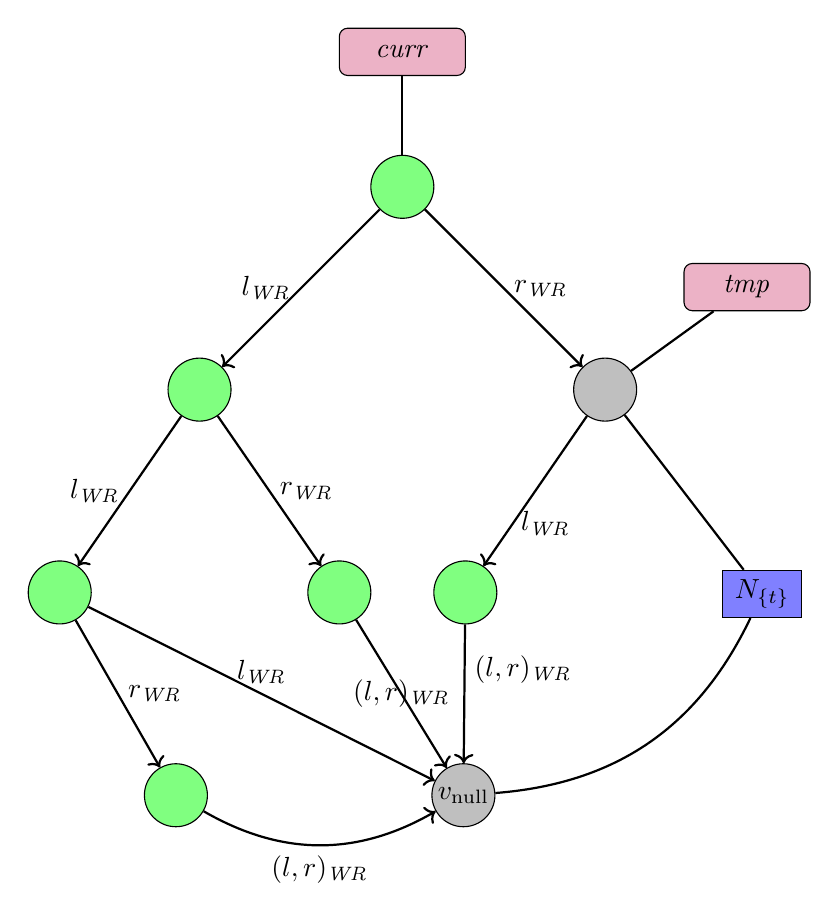
\begin{tikzpicture}[node distance=2 and 2]
	\node[node] (r)  {};
	\node[var] (curr) [above=of r] {$\mathit{curr}$};
	\node[node] (r-l) [below left=of r] {};
	\node[node, fill=gray!50] (r-r) [below right=of r] {};
	\node[node, node distance=2 and 1.2] (r-l-l) [below left=of r-l] {};
	\node[node, node distance=2 and 1.2] (r-l-r) [below right=of r-l] {};
	\node[node, node distance=2 and 1.2] (r-r-l) [below left=of r-r] {};
	\node[node, node distance=2 and 0.9] (r-l-l-r) [below right=of r-l-l] {};
	\node[node, below right=2 and 1 of r-l-r, fill=gray!50] (null) {$v_{\text{null}}$};
	\node[var] (tmp)  [above right=of r-r] {$\mathit{tmp}$};
	\node[he] (p) [below right=2 and 1.2 of r-r] {$N_{\{t\}}$};
	\draw [connector] (tmp) to (r-r);
	\draw [connector] (curr) to (r);
	\draw [connector] (p) to (r-r);
	\draw [connector, bend left] (p) to (null);
	\draw [sel] (r) to node[left]{$l_{\mathit{WR}}$} (r-l) ;
	\draw [sel] (r) to node[right]{$r_{\mathit{WR}}$} (r-r);
	\draw [sel] (r-l) to node[left]{$l_{\mathit{WR}}$} (r-l-l);
	\draw [sel] (r-l) to node[right]{$r_{\mathit{WR}}$} (r-l-r);
	\draw [sel] (r-r) to node[right, label={[label distance=0mm]-90:$l_{\mathit{WR}}$}]{} (r-r-l);
	\draw [sel] (r-l-l) to node[right]{$r_{\mathit{WR}}$} (r-l-l-r);
	\draw [sel] (r-l-l) to node[above]{$l_{\mathit{WR}}$} (null);
	\draw [sel] (r-l-r) to node{$(l,r)_{\mathit{WR}}$} (null);
	\draw [sel] (r-r-l) to node[above right]{$(l,r)_{\mathit{WR}}$} (null);
	\draw [sel, bend right] (r-l-l-r) to node[below]{$(l,r)_{\mathit{WR}}$} (null);
\end{tikzpicture}
}}
			\only<5>{\resizebox{\textwidth}{!}{\input{tikz/forkexample7}}}
		\end{overlayarea}
	\end{columns}
\end{frame}

\begin{frame}
	\frametitle{Initial Heap State}
	\begin{columns}
		\column{0.5\textwidth}
			\begin{equation*}
				\parbox{2cm}{\resizebox{2cm}{!}{\input{tikz/precFork2}}}
			\end{equation*}
			\begin{itemize}
				\item initial heap state for forked program:
					\begin{itemize}
						\item mirror precondition
						\item $\mathit{WR}$ permissions for selectors in alternable
							set
						\item $\mathit{RD}$ permissions for other selectors
						\item set formal parameters
					\end{itemize}
			\end{itemize}
		\column{0.5\textwidth}
			\only<2>{\resizebox{0.7\textwidth}{!}{\begin{tikzpicture}
	\node[node, ext] (r-r) [below right=of r] {$v_{1}$};
	\node[node, node distance=2 and 1.2] (r-r-l) [below left=of r-r] {$v_{2}$};
	\node[node, node distance=2 and 1.2] (r-r-r) [below right=of r-r] {$v_{3}$};
	\node[node]                          (r-r-r-r) [below=of r-r-r] {$v_{4}$};
	\node[node, ext, node distance=3 and 1.2] (null)    [below=of r-r] {$v_{\textbf{null}}$};
	\node[var, above=of r-r] (fp) {$\fp_{1}$};
	\draw [sel] (r-r) to node[right, label={[label distance=0mm]180:$l_{\mathit{RD}}$}]{} (r-r-l);
	\draw [sel] (r-r) to node[right]{$r_{\mathit{WR}}$} (r-r-r);
	\draw [sel] (r-r-r) to node[right]{$r_{\mathit{WR}}$} (r-r-r-r);
	\draw [sel] (r-r-r) to node[above left]{$l_{\mathit{WR}}$} (null);
	\draw [sel, bend left] (r-r-l) to node[above]{$r_{\mathit{RD}}$} (null);
	\draw [sel, bend right] (r-r-l) to node[below]{$l_{\mathit{RD}}$} (null);
	\draw [sel] (r-r-r-r) to node[above]{$r_{\mathit{WR}}$} (null);
	\draw [sel, bend left] (r-r-r-r) to node[below]{$l_{\mathit{WR}}$} (null);
	\draw [connector] (fp) to (r-r);
\end{tikzpicture}
}}
	\end{columns}
\end{frame}

\begin{frame}
	\frametitle{Join}
	\begin{columns}
		\column{0.33\textwidth}
			\begin{equation*}
				\alt<1-2>{\alt<1>{\left(\parbox{2cm}{\resizebox{2cm}{!}{
					\input{tikz/precondition}}}, \{e_2,e_3,e_4, e_7, e_8\},
			\parbox{2cm}{\resizebox{2cm}{!}{\input{tikz/postcondition}}}\right)}
			{\left(\parbox{2cm}{\resizebox{2cm}{!}{
					\input{tikz/precFork3}}}, \{e_2,e_3,e_4, e_7, e_8\},
			\parbox{2cm}{\resizebox{2cm}{!}{\input{tikz/postFork}}}\right)}
				}{
					\parbox{2cm}{\resizebox{2cm}{!}{\input{tikz/postFork}}}
				}
			\end{equation*}
		\column{0.33\textwidth}
		\visible<4->{\parbox{2cm}{\resizebox{2cm}{!}{\begin{tikzpicture}
	\node[node, ext] (r-r) [below right=of r] {$v_{1}$};
	\node[node, node distance=2 and 1.2] (r-r-l) [below left=of r-r] {$v_{2}$};
	\node[node, node distance=2 and 1.2] (r-r-r) [below right=of r-r] {$v_{3}$};
	\node[node]                          (r-r-r-r) [below=of r-r-r] {$v_{4}$};
	\node[node, ext, node distance=3 and 1.2] (null)    [below=of r-r] {$v_{\textbf{null}}$};

	\draw [sel] (r-r) to node[right, label={[label distance=0mm]180:$l_{\mathit{RD}}$}]{$e_{1}$} (r-r-l);
	\draw [sel, bend left] (r-r-l) to node[above, label={[]-90:$e_{5}$}]{$r_{\mathit{RD}}$} (null);
	\draw [sel, bend right] (r-r-l) to node[below, label={[]90:$e_{6}$}]{$l_{\mathit{RD}}$} (null);
\end{tikzpicture}
}}}
		\column{0.33\textwidth}
		\visible<5->{\parbox{2cm}{\resizebox{2cm}{!}{\begin{tikzpicture}
	\node[node, ext] (r-r) [below right=of r] {$v_{1}$};
	\node[node, node distance=2 and 1.2] (r-r-l) [below left=of r-r] {$v_{2}$};
	\node[node, node distance=2 and 1.2] (r-r-r) [below right=of r-r] {$v_{3}$};
	\node[node]                          (r-r-r-r) [below=of r-r-r] {$v_{4}$};
	\node[node, ext, node distance=3 and 1.2] (null)    [below=of r-r] {$v_{\textbf{null}}$};

	\draw [sel] (r-r) to node[right, label={180:$e_{2}$}]{$r_{\mathit{WR}}$} (r-r-r);
	\draw [sel] (r-r-r) to node[right, label={180:$e_{3}$}]{$l_{\mathit{WR}}$} (r-r-r-r);
	\draw [sel] (r-r-r) to node[above left, label={[label distance=-2mm]0:$e_{4}$}]{$r_{\mathit{WR}}$} (null);
	\draw [sel] (r-r-r-r) to node[above,label={[label distance=-1mm]-90:$e_{7}$}]{$r_{\mathit{WR}}$} (null);
	\draw [sel, bend left] (r-r-r-r) to node[below, label={[label distance=-2mm]180:$e_{8}$}]{$l_{\mathit{WR}}$} (null);
\end{tikzpicture}
}}}
	\end{columns}
	\begin{itemize}
		\item re-integrate postcondition upon join:
			\begin{enumerate}
				\item \alert<2>{drop all process identifier}
				\item \alert<4>{return read ticket:}
					\begin{itemize}
						\item<4-> all edges return full $\mathit{RD}$ permission
							$\rightarrow$ read ticket can be returned
						\item<4-> one edge can only return $\mathit{RD}^{\ast}$
							permission $\rightarrow$ read ticket is lost
					\end{itemize}
				\item \alert<5>{return write ticket:}
					\begin{itemize}
						\item<5> return $\mathit{WR}/\mathit{WR}^{\ast}$-part by
							replacing the placeholder
					\end{itemize}
			\end{enumerate}
	\end{itemize}
\end{frame}

\begin{frame}
	\frametitle{Example}
	\begin{columns}
		\column{0.4\textwidth}
		\begin{equation*}
		\alt<1>{\parbox{2cm}{\resizebox{2cm}{!}{\input{tikz/postFork}}}
		}{\alt<2-3>{
			\parbox{2cm}{\resizebox{2cm}{!}{\begin{tikzpicture}
	\node[node, ext] (r-r) [below right=of r] {$v_{1}$};
	\node[node, node distance=2 and 1.2] (r-r-l) [below left=of r-r] {$v_{2}$};
	\node[node, node distance=2 and 1.2] (r-r-r) [below right=of r-r] {$v_{3}$};
	\node[node]                          (r-r-r-r) [below=of r-r-r] {$v_{4}$};
	\node[node, ext, node distance=3 and 1.2] (null)    [below=of r-r] {$v_{\textbf{null}}$};

	\draw [sel] (r-r) to node[right, label={[label distance=0mm]180:$l_{\mathit{RD}}$}]{$e_{1}$} (r-r-l);
	\draw [sel, bend left] (r-r-l) to node[above, label={[]-90:$e_{5}$}]{$r_{\mathit{RD}}$} (null);
	\draw [sel, bend right] (r-r-l) to node[below, label={[]90:$e_{6}$}]{$l_{\mathit{RD}}$} (null);
\end{tikzpicture}
}}}
		{\parbox{2cm}{\resizebox{2cm}{!}{\begin{tikzpicture}
	\node[node, ext] (r-r) [below right=of r] {$v_{1}$};
	\node[node, node distance=2 and 1.2] (r-r-l) [below left=of r-r] {$v_{2}$};
	\node[node, node distance=2 and 1.2] (r-r-r) [below right=of r-r] {$v_{3}$};
	\node[node]                          (r-r-r-r) [below=of r-r-r] {$v_{4}$};
	\node[node, ext, node distance=3 and 1.2] (null)    [below=of r-r] {$v_{\textbf{null}}$};

	\draw [sel] (r-r) to node[right, label={180:$e_{2}$}]{$r_{\mathit{WR}}$} (r-r-r);
	\draw [sel] (r-r-r) to node[right, label={180:$e_{3}$}]{$l_{\mathit{WR}}$} (r-r-r-r);
	\draw [sel] (r-r-r) to node[above left, label={[label distance=-2mm]0:$e_{4}$}]{$r_{\mathit{WR}}$} (null);
	\draw [sel] (r-r-r-r) to node[above,label={[label distance=-1mm]-90:$e_{7}$}]{$r_{\mathit{WR}}$} (null);
	\draw [sel, bend left] (r-r-r-r) to node[below, label={[label distance=-2mm]180:$e_{8}$}]{$l_{\mathit{WR}}$} (null);
\end{tikzpicture}
}}}}
		\end{equation*}
		\begin{enumerate}
			\item \textcolor{black!40}{drop process identifier}
			\item<2-> \alert<2-3>{return read ticket}
			\item<4-5> \alert<4-5>{return $\mathit{WR}$-part}
		\end{enumerate}
		\column{0.6\textwidth}
			\begin{overlayarea}{\textwidth}{\textheight}
				\only<1-2>{\resizebox{0.7\textwidth}{!}{\input{tikz/forkexample7}}}
				\only<3>{\resizebox{0.7\textwidth}{!}{\input{tikz/forkexample8}}}
				\only<4>{\resizebox{0.7\textwidth}{!}{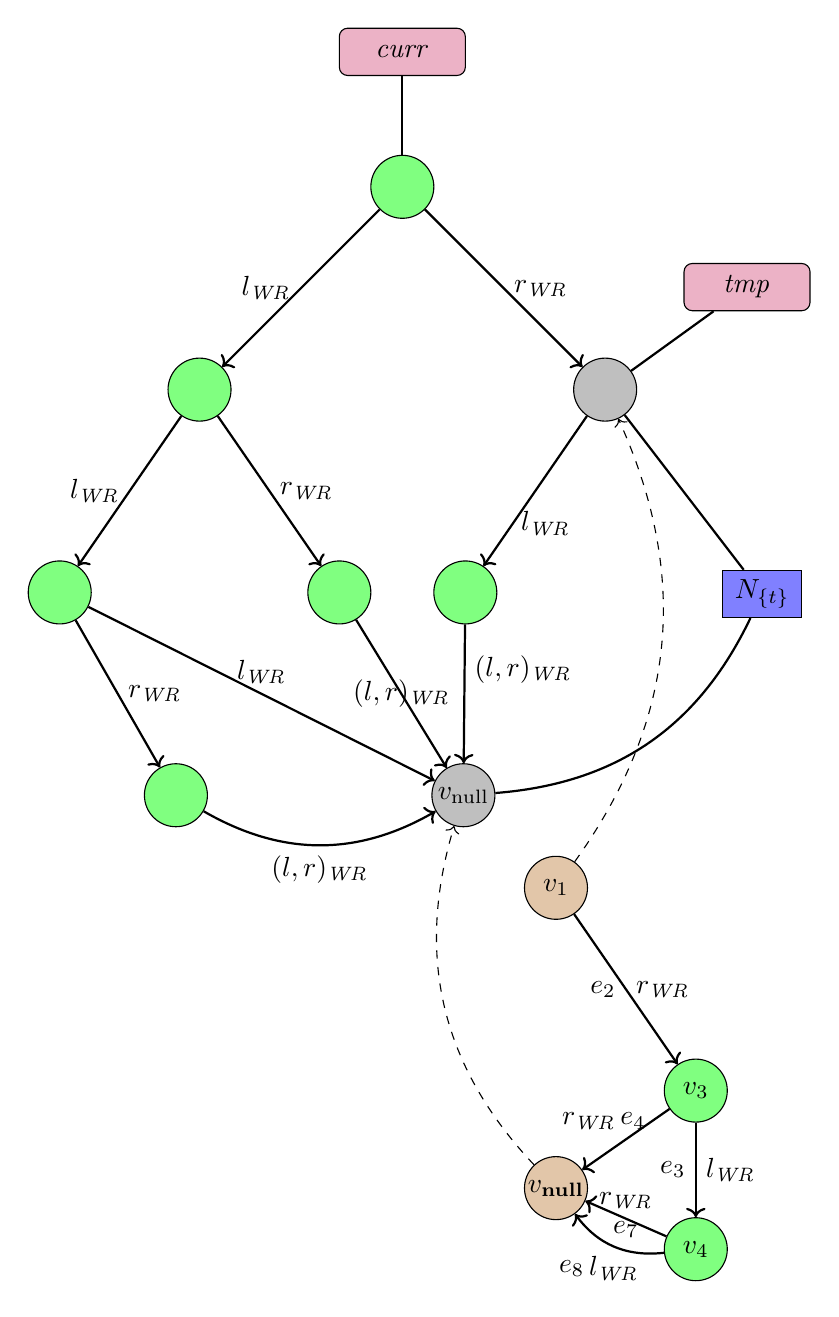
\begin{tikzpicture}[node distance=2 and 2]
	\node[node] (r)  {};
	\node[var] (curr) [above=of r] {$\mathit{curr}$};
	\node[node] (r-l) [below left=of r] {};
	\node[node, fill=gray!50] (r-r) [below right=of r] {};
	\node[node, node distance=2 and 1.2] (r-l-l) [below left=of r-l] {};
	\node[node, node distance=2 and 1.2] (r-l-r) [below right=of r-l] {};
	\node[node, node distance=2 and 1.2] (r-r-l) [below left=of r-r] {};
	\node[node, node distance=2 and 0.9] (r-l-l-r) [below right=of r-l-l] {};
	\node[node, below right=2 and 1 of r-l-r, fill=gray!50] (null) {$v_{\text{null}}$};
	\node[var] (tmp)  [above right=of r-r] {$\mathit{tmp}$};
	\node[he] (p) [below right=2 and 1.2 of r-r] {$N_{\{t\}}$};
	
	\node[node, ext] (r-r2) [below right =0.6 and 0.6 of null] {$v_{1}$};
	\node[node, node distance=2 and 1.2] (r-r-r) [below right=of r-r2] {$v_{3}$};
	\node[node]                          (r-r-r-r) [below=1.2 and 1.2 of r-r-r] {$v_{4}$};
	\node[node, ext, node distance=3 and 1.2] (null2)    [below=of r-r2] {$v_{\textbf{null}}$};

	\draw [sel] (r-r2) to node[right, label={180:$e_{2}$}]{$r_{\mathit{WR}}$} (r-r-r);
	\draw [sel] (r-r-r) to node[right, label={180:$e_{3}$}]{$l_{\mathit{WR}}$} (r-r-r-r);
	\draw [sel] (r-r-r) to node[above left, label={[label distance=-2mm]0:$e_{4}$}]{$r_{\mathit{WR}}$} (null2);
	\draw [sel] (r-r-r-r) to node[above,label={[label distance=-1mm]-90:$e_{7}$}]{$r_{\mathit{WR}}$} (null2);
	\draw [sel, bend left] (r-r-r-r) to node[below, label={[label distance=-2mm]180:$e_{8}$}]{$l_{\mathit{WR}}$} (null2);

	\draw [connector] (tmp) to (r-r);
	\draw [connector] (curr) to (r);
	\draw [connector] (p) to (r-r);
	\draw [connector, bend left] (p) to (null);
	\draw [sel] (r) to node[left]{$l_{\mathit{WR}}$} (r-l) ;
	\draw [sel] (r) to node[right]{$r_{\mathit{WR}}$} (r-r);
	\draw [sel] (r-l) to node[left]{$l_{\mathit{WR}}$} (r-l-l);
	\draw [sel] (r-l) to node[right]{$r_{\mathit{WR}}$} (r-l-r);
	\draw [sel] (r-r) to node[right, label={[label distance=0mm]-90:$l_{\mathit{WR}}$}]{} (r-r-l);
	\draw [sel] (r-l-l) to node[right]{$r_{\mathit{WR}}$} (r-l-l-r);
	\draw [sel] (r-l-l) to node[above]{$l_{\mathit{WR}}$} (null);
	\draw [sel] (r-l-r) to node{$(l,r)_{\mathit{WR}}$} (null);
	\draw [sel] (r-r-l) to node[above right]{$(l,r)_{\mathit{WR}}$} (null);
	\draw [sel, bend right] (r-l-l-r) to node[below]{$(l,r)_{\mathit{WR}}$} (null);

	\draw [->, dashed, bend right] (r-r2) to (r-r);
	\draw [->, dashed, bend left] (null2) to (null);
\end{tikzpicture}
}}
				\only<5>{\resizebox{\textwidth}{!}{\input{tikz/forkexample10}}}
			\end{overlayarea}
	\end{columns}
\end{frame}

\begin{frame}
	\frametitle{Data Race Freedom}
	\begin{theorem}[Data Race Freedom]
		All executions that can be modelled by the presented semantics are data race
		free.
	\end{theorem}
	\begin{itemize}
		\item<2-> by induction over the transition relation it can be shown that for
			sound contracts:
			\begin{enumerate}
				\item<3-> only selectors with a $\mathit{WR}-\emptyset$ permission are
					altered
				\item<4-> write tickets are completely transferred
				\item<5-> for all permissions with $\mathit{WR}$ or $\mathit{RD}$ all
					derived access tickets are properly accounted in the
					$\mathit{PermSets}$
			\end{enumerate}
	\end{itemize}
\end{frame}

\section{Abstraction \& Concretisation}
\begin{frame}
	\frametitle{Idea}
	\begin{itemize}
		\item data structures often share repetetive structure
	\end{itemize}
	\begin{columns}
			\column{0.33\textwidth}
				\resizebox{\textwidth}{!}{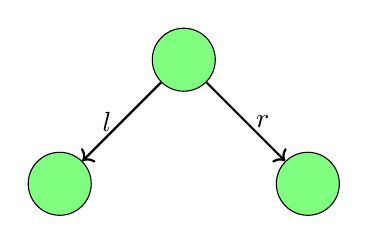
\begin{tikzpicture}
	\node[node] (v1) {};
	\node[node, below left= of v1] (v2) {};
	\node[node, below right=of v1] (v3) {};

	\draw[sel] (v1) to node[left] {$l$} (v2);
	\draw[sel] (v1) to node[right]{$r$} (v3);
\end{tikzpicture}
}
			\column{0.33\textwidth}
				\resizebox{\textwidth}{!}{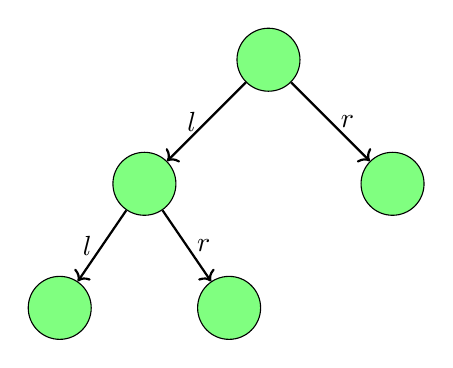
\begin{tikzpicture}
	\node[node] (v1) {};
	\node[node, below left= of v1] (v2) {};
	\node[node, below right=of v1] (v3) {};
	\node[node, below right=1 and 0.5 of v2] (v4) {};
	\node[node, below left=1 and 0.5 of v2] (v5) {};

	\draw[sel] (v1) to node[left] {$l$} (v2);
	\draw[sel] (v1) to node[right]{$r$} (v3);
	\draw[sel] (v2) to node[left] {$l$} (v5);
	\draw[sel] (v2) to node[right] {$r$} (v4);
\end{tikzpicture}
}
			\column{0.33\textwidth}
				\resizebox{\textwidth}{!}{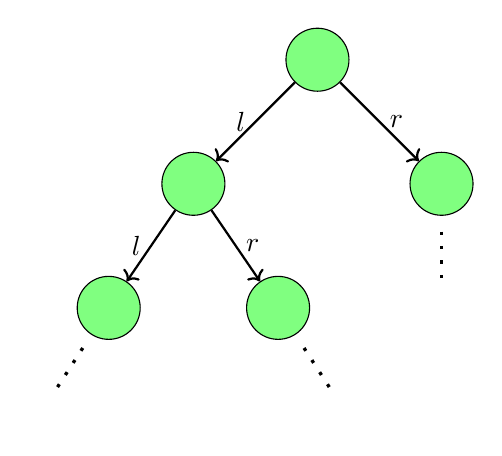
\begin{tikzpicture}
	\node[node] (v1) {};
	\node[node, below left= of v1] (v2) {};
	\node[node, below right=of v1] (v3) {};
	\node[node, below right=1 and 0.5 of v2] (v4) {};
	\node[node, below left=1 and 0.5 of v2] (v5) {};
	\node[below left=1 and 0.5 of v5] (dots1) {};
	\node[below right=1 and 0.5 of v4] (dots2) {};
	\node[below=1 and 0.5 of v3] (dots3) {};

	\draw[sel] (v1) to node[left] {$l$} (v2);
	\draw[sel] (v1) to node[right]{$r$} (v3);
	\draw[sel] (v2) to node[left] {$l$} (v5);
	\draw[sel] (v2) to node[right] {$r$} (v4);
	\draw[loosely dotted, very thick, shorten >= 0.2cm, shorten <= 0.2cm] (v5) to (dots1);
	\draw[loosely dotted, very thick, shorten >= 0.2cm, shorten <= 0.2cm] (v4) to (dots2);
	\draw[loosely dotted, very thick, shorten >= 0.2cm, shorten <= 0.2cm] (v3) to (dots3);
\end{tikzpicture}
}
	\end{columns}
	\begin{itemize}
		\item[$\Rightarrow$] represent structure of arbitrary size as \emph{one}
			hyperedge from which the different structures can be derived on demand
		\item introduce \emph{nonterminals} as representing hyperedges
		\item set of production rules to derive structures $\rightarrow$
			\emph{hyperedge replacement grammars} (HRGs)
	\end{itemize}
\end{frame}

\begin{frame}
	\frametitle{Permissions in HRGs}
	\begin{itemize}
		\item permission propagate strictly through application of production rules:
			\begin{itemize}
				\item all edges of right hand sides have the same permission
				\item \parbox{4cm}{\resizebox{4cm}{!}{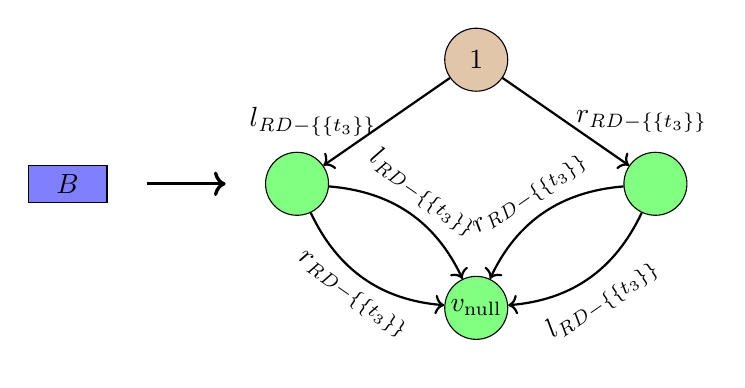
\begin{tikzpicture}
	\node[he] (lhs) {$B$};
	\node[node, right=1cm and 2cm of lhs] (v2) {};
	\node[node, ext, above right=1 and 1.7 of v2] (v1) {$1$};
	\node[node, below right=1 and 1.7 of v1] (v3) {};
	\node[node, below right=1 and 1.7 of v2] (null) {$v_{\text{null}}$};

	\draw[very thick, ->, shorten >=0.5cm, shorten <=0.5cm] (lhs) to (v2);
	\draw[sel] (v1) to node[left] {$l_{\mathit{RD}-\{\{t_3\}\}}$} (v2);
	\draw[sel] (v1) to node[right]{$r_{\mathit{RD}-\{\{t_3\}\}}$} (v3);
	\draw[sel, bend left, sloped] (v2) to node[above]{$l_{\mathit{RD}-\{\{t_3\}\}}$} (null);
	\draw[sel, bend right, sloped] (v2) to node[below]{$r_{\mathit{RD}-\{\{t_3\}\}}$} (null);
	\draw[sel, bend left, sloped] (v3) to node[below]{$l_{\mathit{RD}-\{\{t_3\}\}}$} (null);
	\draw[sel, bend right, sloped] (v3) to node[above]{$r_{\mathit{RD}-\{\{t_3\}\}}$} (null);
\end{tikzpicture}
}}
				\item production rules can only be applied to nonterminals with the
					permission of the right hand side
			\end{itemize}
		\item separate structure and permission:
	\end{itemize}
	\begin{definition}[Fully Permissive Grammar]
		$G\in\HRG$ is called \emph{fully permissive} if the following holds:
		Every production rule $p\colon X\rightarrow H$ in $G$ exists for every
		$\rho\in\PES$.
	\end{definition}
\end{frame}

\begin{frame}
	\frametitle{Example}
	$\left\{\begin{aligned}
			 & \parbox{2.5cm}{\resizebox{2.5cm}{!}{
					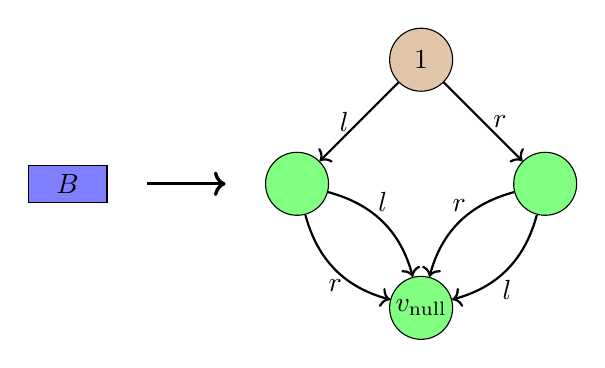
\begin{tikzpicture}
	\node[he] (lhs) {$B$};
	\node[node, right=1cm and 2cm of lhs] (v2) {};
	\node[node, ext, above right=of v2] (v1) {$1$};
	\node[node, below right=of v1] (v3) {};
	\node[node, below right=of v2] (null) {$v_{\text{null}}$};

	\draw[very thick, ->, shorten >=0.5cm, shorten <=0.5cm] (lhs) to (v2);
	\draw[sel] (v1) to node[left] {$l$} (v2);
	\draw[sel] (v1) to node[right]{$r$} (v3);
	\draw[sel, bend left] (v2) to node[above]{$l$} (null);
	\draw[sel, bend right] (v2) to node[below]{$r$} (null);
	\draw[sel, bend left] (v3) to node[below]{$l$} (null);
	\draw[sel, bend right] (v3) to node[above]{$r$} (null);
\end{tikzpicture}

				}}, \parbox{2.5cm}{\resizebox{2.5cm}{!}{
					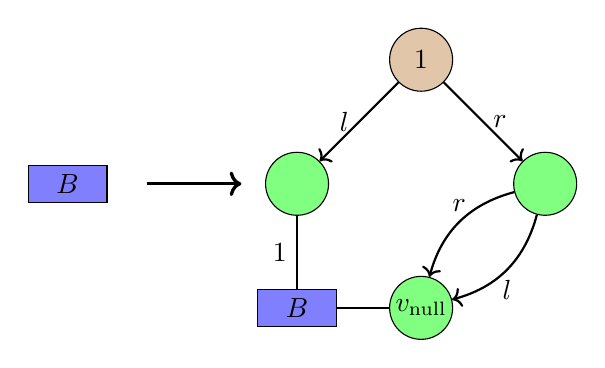
\begin{tikzpicture}
	\node[he] (lhs) {$B$};
	\node[node, right=1cm and 2cm of lhs] (v2) {};
	\node[node, ext, above right=of v2] (v1) {$1$};
	\node[node, below right=of v1] (v3) {};
	\node[node, below right=of v2] (null) {$v_{\text{null}}$};
	\node[he] (e1) at (null-|v2) {$B$};

	\draw[very thick, ->, shorten >=0.3cm, shorten <=0.5cm] (lhs) to (v2);
	\draw[sel] (v1) to node[left] {$l$} (v2);
	\draw[sel] (v1) to node[right]{$r$} (v3);
	\draw[connector] (v2) to node[left]{$1$} (e1);
	\draw[sel, bend left] (v3) to node[below]{$l$} (null);
	\draw[sel, bend right] (v3) to node[above]{$r$} (null);
	\draw[connector] (e1) to (null);
\end{tikzpicture}

				}},\\& \parbox{2.5cm}{\resizebox{2.5cm}{!}{
					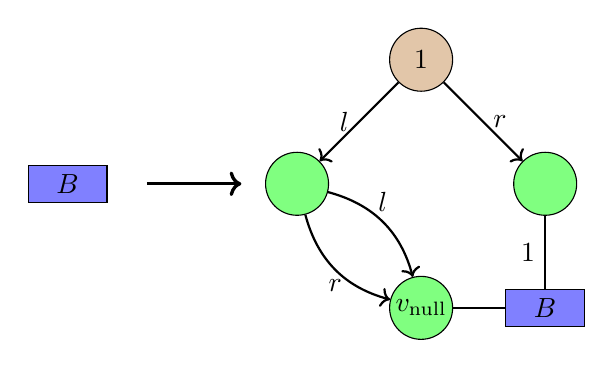
\begin{tikzpicture}
	\node[he] (lhs) {$B$};
	\node[node, right=1cm and 2cm of lhs] (v2) {};
	\node[node, ext, above right=of v2] (v1) {$1$};
	\node[node, below right=of v1] (v3) {};
	\node[node, below right=of v2] (null) {$v_{\text{null}}$};
	\node[he] (e1) at (null-|v3) {$B$};

	\draw[very thick, ->, shorten >=0.3cm, shorten <=0.5cm] (lhs) to (v2);
	\draw[sel] (v1) to node[left] {$l$} (v2);
	\draw[sel] (v1) to node[right]{$r$} (v3);
	\draw[connector] (v3) to node[left]{$1$} (e1);
	\draw[sel, bend left] (v2) to node[above]{$l$} (null);
	\draw[sel, bend right] (v2) to node[below]{$r$} (null);
	\draw[connector] (e1) to (null);
\end{tikzpicture}

				}}, \parbox{2.5cm}{\resizebox{2.5cm}{!}{
					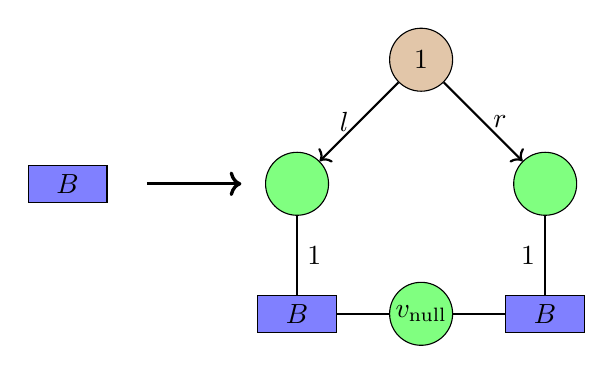
\begin{tikzpicture}
	\node[he] (lhs) {$B$};
	\node[node, right=1cm and 2cm of lhs] (v2) {};
	\node[node, ext, above right=of v2] (v1) {$1$};
	\node[node, below right=of v1] (v3) {};
	\node[he, below=of v3] (e2) {$B$};
	\node[he, below=of v2] (e1) {$B$};
	\node[node] (null) at (e1-|v1) {$v_{\text{null}}$};

	\draw[very thick, ->, shorten >=0.3cm, shorten <=0.5cm] (lhs) to (v2);
	\draw[sel] (v1) to node[left] {$l$} (v2);
	\draw[sel] (v1) to node[right]{$r$} (v3);
	\draw[connector] (v3) to node[left]{$1$} (e2);
	\draw[connector] (v2) to node[right]{$1$} (e1);
	\draw[connector] (e1) to (null);
	\draw[connector] (e2) to (null);
\end{tikzpicture}

		}}
		\end{aligned} \right\}$
	\flushright\scalebox{0.4}{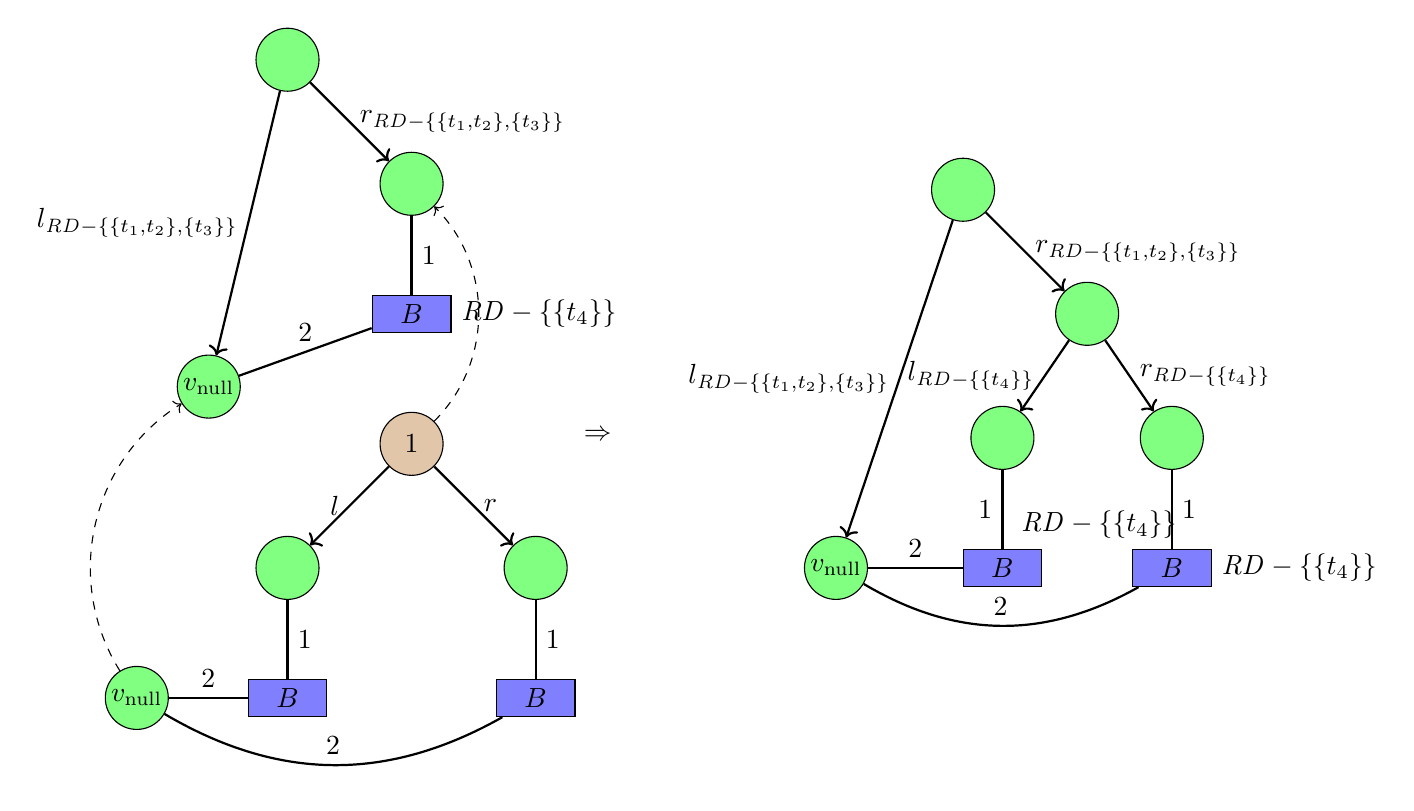
\begin{tikzpicture}
	%graph
	\node[node] (s1) {};
	\node[node, below right=of s1] (s3) {};
	\node[node, node distance=2 and 2, below left =of s3] (s2) {$v_{\text{null}}$};
	\node[he, below=of s3, label={[]0:$\mathit{RD}-\{\{t_4\}\}$}] (e3) {$B$};

	\draw[sel] (s1) to node[left ]{$l_{\mathit{RD}-\{\{t_1,t_2\}, \{t_3\}\}}$} (s2);
	\draw[sel] (s1) to node[right]{$r_{\mathit{RD}-\{\{t_1,t_2\}, \{t_3\}\}}$} (s3);
	\draw[connector] (e3) to node[above]{2} (s2);
	\draw[connector] (e3) to node[right]{1} (s3);

	%rhs of production rule:
	\visible<2->{\node[node, below=of e3, ext] (v1) {1};
	\node[node, below left=of v1] (v2) {};
	\node[node, below right=of v1] (v3) {};
	\node[he, below=of v2] (e1) {$B$};
	\node[he, below=of v3] (e2) {$B$};
	\node[node, left=of e1] (v4) {$v_{\text{null}}$};

	\draw[sel] (v1) to node[left ]{$l$} (v2);
	\draw[sel] (v1) to node[right]{$r$} (v3);
	\draw[connector] (e1) to node[right]{1} (v2);
	\draw[connector] (e1) to node[above]{2} (v4);
	\draw[connector, bend left] (e2) to node[above]{2} (v4);
	\draw[connector] (e2) to node[right]{1} (v3);

	%connection
	\draw[dashed, ->, bend right=45] (v1) to (s3);
	\draw[dashed, ->, bend left=45]  (v4) to (s2);}

	%leadsto symbol
	\visible<3->{\node[above right=1.2cm and 0.2cm of v3] {$\Rightarrow$};

	%result
		\node[node] (null) [right=3 and 3 of v3] {$v_{\text{null}}$};
	\node[he] (e1) [right=1.2 and 1.2 of null, label={[]65:$\mathit{RD}-\{\{t_4\}\}$}] {$B$};
	\node[node, above=of e1] (root-right-left) {};
	\node[node, above right=1cm and 0.5cm of root-right-left](root-right){};
	\node[node, below right=1cm and 0.5cm of root-right](root-right-right){};
	\node[node, above left=of root-right] (root) {};
	\node[he, below=of root-right-right, label={[]0:$\mathit{RD}-\{\{t_4\}\}$}] (e2) {$B$};

	\draw[sel] (root) to node[right]{$r_{\mathit{RD}-\{\{t_1,t_2\}, \{t_3\}\}}$} (root-right);
	\draw[sel] (root) to node[left ]{$l_{\mathit{RD}-\{\{t_1,t_2\}, \{t_3\}\}}$} (null);
	\draw[sel] (root-right) to node[left ]{$l_{\mathit{RD}-\{\{t_4\}\}}$} (root-right-left);
	\draw[sel] (root-right) to node[right]{$r_{\mathit{RD}-\{\{t_4\}\}}$} (root-right-right);
	\draw[connector] (e1) to node[left ]{1} (root-right-left);
	\draw[connector] (e2) to node[right]{1} (root-right-right);
	\draw[connector] (e1) to node[above]{2} (null);
	\draw[connector, bend left] (e2) to node[above]{2} (null);}

\end{tikzpicture}
}
\end{frame}

\begin{frame}
	\frametitle{Abstraction}
	\begin{itemize}
		\item parts of heap representations can be abstracted by applying
			production rules backwards
		\item permission of introduced nonterminal fits permission of abstracted
			subgraph
	\end{itemize}
	\resizebox{\textwidth}{!}{\input{tikz/bintreeabspres}}
\end{frame}

\begin{frame}
	\frametitle{Semantics}
	\begin{itemize}
		\item concrete semantics for pointer operations can be applied to
			partially abstract hypergraphs as long all accessible selectors
			are present
		\item Recall: for pointer operations the depth of dereferences is $1$
	\end{itemize}
	\begin{columns}
		\column{0.5\textwidth}
			\begin{overlayarea}{\textwidth}{\textheight}
				\scalebox{0.8}{\resizebox{\textwidth}{!}{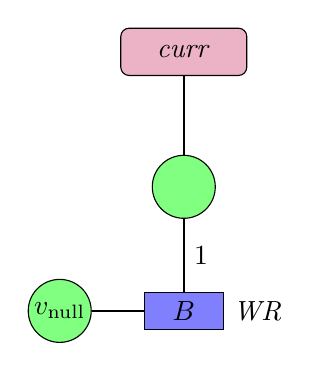
\begin{tikzpicture}
	\node[var]                 (curr) {$\mathit{curr}$};
	\node[node, below=of curr] (v)    {};
	\node[node, below left=of v] (null) {$v_{\text{null}}$};
	\node[he, label={0:{$\mathit{WR}$}}] (e) at (null-|v) {$B$};

	\draw[connector] (curr) to                  (v);
	\draw[connector] (e)    to node[right]{$1$} (v);
	\draw[connector] (e)    to                  (null);
\end{tikzpicture}
}}
			\end{overlayarea}
		\column{0.5\textwidth}
			\begin{overlayarea}{\textwidth}{\textheight}
				\only<2>{\scalebox{0.9}{\resizebox{\textwidth}{!}{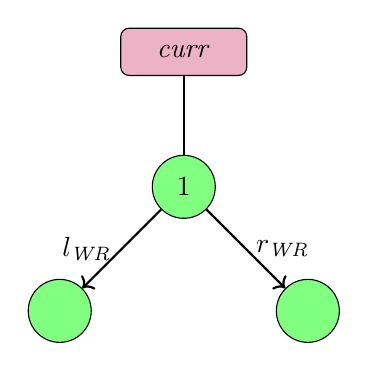
\begin{tikzpicture}
	\node[node] (v1) {$1$};
	\node[node, below left= of v1] (v2) {};
	\node[node, below right=of v1] (v3) {};
	\node[var, above=of v1] (curr) {$\mathit{curr}$};

	\draw[connector] (curr) to (v1);
	\draw[sel] (v1) to node[left] {$l_{\mathit{WR}}$} (v2);
	\draw[sel] (v1) to node[right]{$r_{\mathit{WR}}$} (v3);
\end{tikzpicture}
}}}
				\only<3>{\scalebox{0.9}{\resizebox{\textwidth}{!}{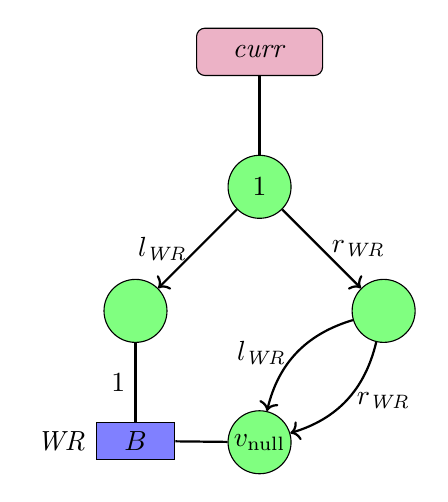
\begin{tikzpicture}
	\node[var] (curr) {$\mathit{curr}$};
	\node[node, below=of curr] (v1) {$1$};
	\node[node, below left= of v1] (v2) {};
	\node[node, below right=of v1] (v3) {};
	\node[he, below=of v2, label=180:{$\mathit{WR}$}] (e1) {$B$};
	\node[node, below=2.43 and 2 of v1] (null) {$v_{\text{null}}$};

	\draw[sel] (v1) to node[left] {$l_{\mathit{WR}}$} (v2);
	\draw[sel] (v1) to node[right]{$r_{\mathit{WR}}$} (v3);
	\draw[connector] (v2) to node[left]{$1$} (e1);
	\draw[connector] (e1) to (null);
	\draw[connector] (curr) to (v1);
	\draw[sel, bend right] (v3) to node[left]{$l_{\mathit{WR}}$} (null);
	\draw[sel, bend left] (v3) to node[right]{$r_{\mathit{WR}}$} (null);
\end{tikzpicture}
}}}
				\only<4>{\scalebox{0.9}{\resizebox{\textwidth}{!}{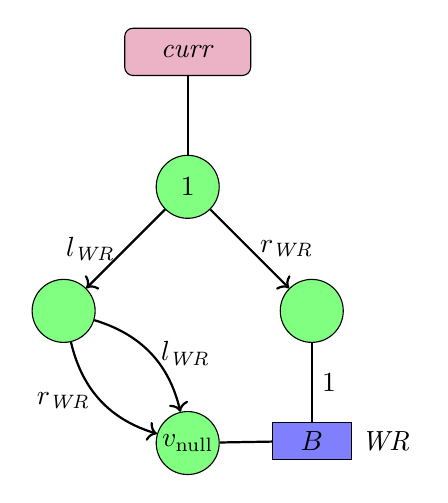
\begin{tikzpicture}
	\node[var] (curr) {$\mathit{curr}$};
	\node[node, below=of curr] (v1) {$1$};
	\node[node, below left=of v1] (v2) {};
	\node[node, below right=of v1] (v3) {};
	\node[he, below=of v3, label=0:{$\mathit{WR}$}] (e1) {$B$};
	\node[node, below=2.44 and 2 of v1] (null) {$v_{\text{null}}$};

	\draw[sel] (v1) to node[left] {$l_{\mathit{WR}}$} (v2);
	\draw[sel] (v1) to node[right]{$r_{\mathit{WR}}$} (v3);
	\draw[connector] (v3) to node[right]{$1$} (e1);
	\draw[connector] (e1) to (null);
	\draw[connector] (curr) to (v1);
	\draw[sel, bend left] (v2) to node[right]{$l_{\mathit{WR}}$} (null);
	\draw[sel, bend right] (v2) to node[left]{$r_{\mathit{WR}}$} (null);
\end{tikzpicture}
}}}
				\only<5>{\scalebox{0.9}{\resizebox{\textwidth}{!}{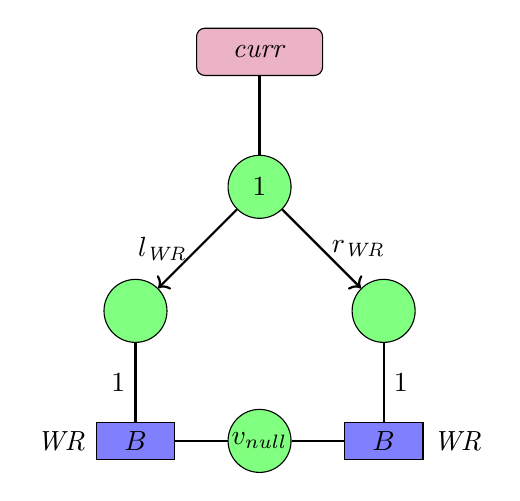
\begin{tikzpicture}
	\node[var] (curr) {$\mathit{curr}$};
	\node[node, below=of curr] (v1) {$1$};
	\node[node, below left=of v1] (v2) {};
	\node[node, below right=of v1] (v3) {};
	\node[he, below=of v3, label=0:{$\mathit{WR}$}] (e2) {$B$};
	\node[he, below=of v2, label=180:{$\mathit{WR}$}] (e1) {$B$};
	\node[node] (null) at (e2-|curr) {$v_{null}$};

	\draw[sel] (v1) to node[left] {$l_{\mathit{WR}}$} (v2);
	\draw[sel] (v1) to node[right]{$r_{\mathit{WR}}$} (v3);
	\draw[connector] (v3) to node[right]{$1$} (e2);
	\draw[connector] (v2) to node[left] {$1$} (e1);
	\draw[connector] (e1) to (null);
	\draw[connector] (e2) to (null);
	\draw[connector] (curr) to (v1);
\end{tikzpicture}
}}}
			\end{overlayarea}
	\end{columns}
\end{frame}

\begin{frame}
	\frametitle{Semantics: Fork}
	\begin{itemize}
		\item adapt concrete semantics:
			\begin{itemize}
				\item \alert<2-3>{abstract contracts:}
					\begin{itemize}
						\item abstract precondition represents multiple heaps
							$\rightarrow$ so does initial heap state
						\item postcondition might depend on concretisation
							$\rightarrow$ multiple postconditions
						\item[$\Rightarrow$] $ \Cont_{\text{abs}}\colon\Proc
							\rightarrow \mathbb{P}(\HGN\times\mathbb{P}(E)\times
							\alert<3>{\mathbb{P}(\mathit{HG}^{\PI'}_{\Sigma_{N}'})})$
					\end{itemize}
				\item \alert<4-5>{reachability over nonterminals:}
					\begin{itemize}
						\item if nonterminal can be concretised to reachability
						\item if nonterminal abstracts reachable parts
						\item<5> (example: \parbox{4cm}{\resizebox{4cm}{!}{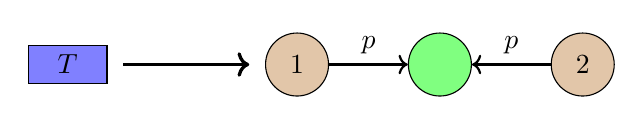
\begin{tikzpicture}
	\node[he] (lhs) {$T$};
	\node[node, ext, right=1cm and 2cm of lhs] (v1) {$1$};
	\node[node, right=of v1] (v2) {};
	\node[node, ext, right=of v2] (v3) {$2$};

	\draw[->, very thick, shorten >=0.2cm, shorten <=0.2cm] (lhs) to (v1);
	\draw[sel] (v1) to node[above]{$p$} (v2);
	\draw[sel] (v3) to node[above]{$p$} (v2);
\end{tikzpicture}
}})
						\item[$\Rightarrow$] include into reachable subgraph
					\end{itemize}
			\end{itemize}
	\end{itemize}
\end{frame}

\begin{frame}
	\frametitle{Semantics: Join}
	\begin{itemize}
		\item adapt concrete semantics:
			\begin{itemize}
				\item join \emph{every} postcondition:
				\item read token returned by permissions only
					\begin{itemize}
						\item no matching between read edges
						\item allows for modular analysis for every process
					\end{itemize}
				\item $\mathit{WR}/\mathit{WR}^{\ast}$-part returned by replacement
					of placeholder
			\end{itemize}
	\end{itemize}
\end{frame}

\begin{frame}
	\frametitle{Over-approximation}
	\begin{theorem}[Overapproximation]
		The abstract semantics are an over-approximation of the concrete
		semantics.
	\end{theorem}
\end{frame}

\begin{frame}
	\frametitle{Proof Intuition}
	\begin{itemize}
		\item contracts: \parbox{7cm}{\resizebox{7cm}{!}{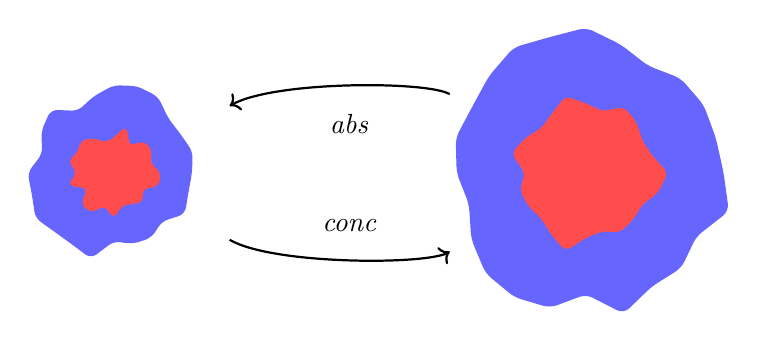
\begin{tikzpicture}
  \coordinate (abs) at (0,0);
  \coordinate (conc) at (6,0);
  \draw[blue!60, fill=blue!60, rounded corners=0.8mm] (abs) \irregularcircle{1cm}{1.5mm};
  \draw[red!70, fill=red!70, rounded corners=0.6mm] (abs) \irregularcircle{0.5cm}{1.2mm};

  \draw[blue!60, fill=blue!60, rounded corners=.9mm] (conc) \irregularcircle{1.7cm}{1.8mm};
  \draw[red!70, fill=red!70, rounded corners=.7mm] (conc) \irregularcircle{0.9cm}{1.5mm};

  \draw[->, thick, shorten <= 1.7cm, shorten >= 2cm, bend right] (abs) to node[above]{$\mathit{conc}$} (conc);
  \draw[->, thick, shorten <= 2cm, shorten >= 1.7cm, bend right] (conc) to node[below]{$\abs$} (abs);
\end{tikzpicture}

}}
		\item contracts: one abstract postcondition concretises to the concrete
			postcondition
		\item compute reachability for concrete hypergraphs in its abstraction
	\end{itemize}
	\begin{equation*}
		\scalebox{0.5}{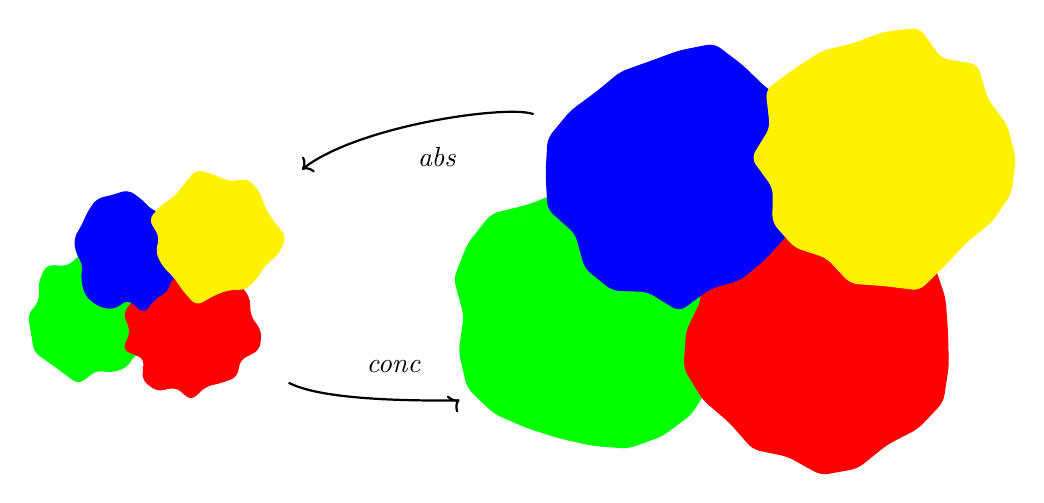
\begin{tikzpicture}
	\coordinate (a1) at (0,0.2);
	\coordinate (a2) at (1.2,0);
	\coordinate (a3) at (0.4,1);
	\coordinate (a4) at (1.5,1.2);

	\draw[green, fill=green, rounded corners=.8mm] (a1) \irregularcircle{0.8cm}{1.2mm};
	\draw[red, fill=red, rounded corners=.8mm] (a2) \irregularcircle{0.8cm}{1.2mm};
	\draw[blue, fill=blue, rounded corners=.8mm] (a3) \irregularcircle{0.7cm}{1.2mm};
	\draw[yellow, fill=yellow, rounded corners=.8mm] (a4) \irregularcircle{0.8cm}{1.2mm};

	\coordinate (c1) at (6.3,0.2);
	\coordinate (c2) at (9.2,0);
	\coordinate (c3) at (7.4,2);
	\coordinate (c4) at (10,2.2);

	\draw[green, fill=green, rounded corners=.9mm] (c1) \irregularcircle{1.7cm}{1.4mm};
	\draw[red, fill=red, rounded corners=.9mm] (c2) \irregularcircle{1.7cm}{1.5mm};
	\draw[blue, fill=blue, rounded corners=.9mm] (c3) \irregularcircle{1.6cm}{1.4mm};
	\draw[yellow, fill=yellow, rounded corners=.9mm] (c4) \irregularcircle{1.6cm}{1.5mm};

	\draw[->, thick, bend right, shorten <= 2cm, shorten >= 1.4cm] (c3) to node[below]{$\abs$} (a4);
	\draw[->, thick, bend right, shorten <= 1.4cm, shorten >= 2cm] (a2) to node[above]{$\mathit{conc}$} (c1);
\end{tikzpicture}
}
	\end{equation*}
	\blfootnote{\cite[pp. 111-115]{HandbookGraphGrammars}, \cite[p. 19]{fmsd}}
\end{frame}

\begin{frame}
	\frametitle{Abstract Data Race Freedom}
	\begin{itemize}
		\item valid modelling of execution by abstract semantics ensures valid
			modelling of execution by all represented concrete semantics
		\item[$\Rightarrow$] all executions are data race free
	\end{itemize}
\end{frame}

\section{Conclusion}
\begin{frame}
	\frametitle{Conclusion}
	\begin{itemize}
		\item incorporate permission model in heap representing hypergraphs
		\item introduced fork \& join
		\item modelled semantics by hypergraph transformations
		\item correct over-approximation by abstracting with hyperedge
			replacement grammars
		\item ensures data race freedom
	\end{itemize}
\end{frame}

\section{Future Work}
\begin{frame}
	\frametitle{Future Work}
	\begin{itemize}
		\item automatic generation of contracts\footnote{like in \cite{ProcedureSummaries}}
		\item integrating into Juggrnaut Tool
		\item treating processes as heap objects
		\item explore other shared resources (e.g. monitor {\cite{Monitor}})
		\item refine under-approximation of permissions ($\mathit{WR}^{\ast},
			\mathit{RD}^{\ast}$ represent logically the same permission)
		\item allow concretisation steps at fork for finer write demands
	\end{itemize}
	\nocite{thesis}
\end{frame}

\section{References}

\metroset{sectionpage=none}
\begin{frame}[allowframebreaks]
	\printbibliography
\end{frame}

\begin{frame}[plain]
	\centering\Huge Thank you for the attention!
\end{frame}

%backup

\end{document}
